\documentclass[11pt]{article}
\usepackage[letterpaper,margin=1in]{geometry}
\usepackage[T1]{fontenc}
\usepackage{mathptmx}
\usepackage[scaled=0.9]{helvet}
\usepackage{microtype}
\usepackage{amsmath,amssymb,bm}
\usepackage{booktabs,tabularx,multirow}
\usepackage{graphicx}
\usepackage[table]{xcolor}
\usepackage{tikz}
\usetikzlibrary{arrows.meta,positioning,calc,shapes.geometric,decorations.pathreplacing}
\usepackage{enumitem}
\usepackage[font=small,labelfont=bf,skip=4pt]{caption}
\usepackage[numbers,sort&compress]{natbib}
\usepackage{xurl}
\usepackage[colorlinks=true,linkcolor=goodblue,citecolor=goodblue,urlcolor=goodblue]{hyperref}

\definecolor{goodblue}{HTML}{2A78D6}
\definecolor{badorange}{HTML}{EB6834}
\definecolor{ntpaqua}{HTML}{1BAF7A}
\definecolor{custA}{HTML}{6250D6}
\definecolor{custB}{HTML}{EDA100}
\definecolor{custC}{HTML}{E87BA4}
\definecolor{inktwo}{HTML}{52514E}

\setlist{itemsep=2pt,topsep=3pt,leftmargin=1.4em}
\setlength{\parskip}{3pt}
\hyphenation{rotation rotations}
\newcommand{\good}{\textcolor{goodblue}{\textbf{good views}}}
\newcommand{\figref}[1]{Figure~\ref{#1}}
\newcommand{\secref}[1]{\S\ref{#1}}

\title{\textbf{Toward World Models of Organizations:\\Every System Sees the Same Company}}
\author{Ashwin Gopinath\\[2pt] \normalsize Sentra, San Francisco}
\date{November 2026}

\begin{document}
\maketitle

\begin{abstract}
\noindent
A company is one world observed by many systems. Email, chat, the CRM, support tickets, call recordings, calendars and issue trackers each record part of what is happening with every customer, deal and project, yet no system records the situation itself. We ask how a machine can learn a \emph{world model of the organization} whose state space places every record by the situation it describes, whichever system wrote it. Our starting point is the Platonic Representation Theorem: joint-embedding predictive architectures (JEPAs) trained on \emph{good views}, different observations of one underlying state, converge to the same representation up to a rotation. Our observation is that organizations already keep good views without anyone annotating them: records that different systems link to the same customer in the same time window. On a simulated company from Era by Eon (seven systems, 21{,}972 customer-linked records, exact ground truth), small text JEPAs trained from scratch on such links place HOGOODCUST of records whose links were hidden with the right customer, against HOTFCUST for TF-IDF, and the same views raise a frozen pretrained sentence encoder from PTRAWHO to PTHEADHO. With the names of customers \emph{and} employees and all identifiers masked, about half of the customer signal remains. Separately trained encoders can be partly aligned by one rotation, and a rotation lets a retrained encoder search the old index. We build access control into the model: secrets planted in records a reader may not read leak through an encoder trained on everything even when search results and states are filtered, and do not leak when each reader's model is trained only on what they may read; a shared pretrained backbone, which holds no company data, recovers part of the accuracy this costs readers who may read little. Beyond the state space, our experiments point to a division of labor among the parts of a world model. In memory, the state space should route a question to its situation and the stored records should supply the detail. When a question names its customer, a store of pretrained-encoder vectors answers as well as any combination of channels. When the question comes instead with one record of the customer and names are kept in the records, placing that record in the state space and reading its customer's records answers ANCHPPLACESTATEACC of the questions, against ANCHPPLACEDETAILACC when a pretrained encoder places it, ANCHPCLOSEDACC with no store and ANCHPLINKACC with the record's own link; with every name masked, only the record's own link helps clearly. Dynamics did not emerge from a space trained for static similarity: with monthly and weekly windows, forecasts, linear dynamics, drift and cross-team distances stay at chance or simple baselines, while similar situations across customers are found at about twice chance. We then build the decision layer on the same space, reading six kinds of logged action, conditioning the predictor on them and simulating decisions for customers in trouble. On logged data it learns little about what decisions do. This month's actions add nothing to predicting next month's state; in the link-trained space, this month's state already encodes most of them. Next month's actions help, but mostly as a description of the records next month's state is built from. And similar past situations return the situations in which the company acted rather than the effect of acting, because it almost always intervened, and in situations unlike those where it held back. We argue that learning from decisions will need actions whose assignment is known. Every encoder and head we timed trains in TRAINMINLO--TRAINMINHI minutes on a CPU, without a GPU, so at this scale a company could retrain its state space and each access scope's model daily, or whenever an access rule changes. We argue that corporate AI will run on an operational world model of this kind, which people and agents can understand the company through, learn on and improve, and we release our code, data exporter and all results.
\end{abstract}

% ============================================================================================ FIGURE 1
\begin{figure}[t]
\centering
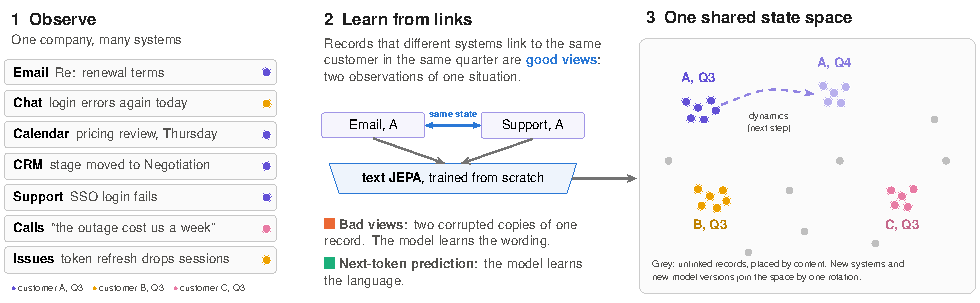
\includegraphics[width=\linewidth]{figures/idea.pdf}
\caption{\textbf{The idea.} (1) Every system records a piece of each customer's situation. (2) The links the systems already keep tell us which records are two observations of the same situation, the \emph{good views} that the Platonic Representation Theorem asks for. (3) A JEPA trained on them maps records from every system into one state space where records about the same customer and quarter land together and records without links can be placed by content; separately trained or retrained encoders can be partly aligned by a rotation. Predicting how states move is the next step toward a full world model.}
\label{fig:idea}
\end{figure}

% ============================================================================================ 1
\section{Introduction}
\label{sec:intro}

Ask anyone in a company what is going on with its largest customer. The honest answer is spread across a sales call last Tuesday, three support tickets, a chat thread, an email chain with procurement and a CRM stage that is two weeks out of date. Each system records a piece of the situation; none records the situation itself. People rebuild it in their heads, slowly, partially and differently from one another. AI assistants rebuild it from scratch every time they are asked, by retrieving documents and reading them.

What is missing is a model of the company itself: a \emph{world model}. In robotics and video, a world model is a learned representation of the state of the world together with a way to predict how that state changes~\citep{ha2018world,hafner2020dreamer,lecun2022path}. For an organization, the world is the situation of every customer, deal, project and team at every moment, and the observations are the records the organization produces as it works. A world model of an organization would map every record, from every system, into one state space where records about the same situation land together. It would stay stable as systems, models and time change. Eventually, it would predict how states evolve and how actions change them.

We think every company will come to run on such a model, and that it is what corporate AI is missing: an \emph{operational world model} that represents how the company actually functions. A capable new employee spends months learning a company from what happens around them: which customers are struggling, which deals are moving, who knows what. An operational world model lets people and AI agents learn the company the same way, from the company's own record of what happened, and lets them try a change against the model before making it in the company. Understanding the company, learning on it, and improving it all start from the same object.

The hard part is learning such a space without labels. Nobody annotates ``situations''. Generic text embeddings organize records by topic and template; next-token prediction learns the language of the records, not the company. The Platonic Representation Theorem~\citep{balestriero2026platonic} makes the requirement precise. JEPAs trained on \good{}, two different observations of the same underlying state, converge to the same representation up to one rotation, whatever the modality. With \emph{bad views}, corruptions of a single observation, they do not, and next-token prediction behaves like a JEPA with bad views. In vision and language, good views are scarce: someone has to pair an image with its caption.

A model of a company has a requirement that a model of the physical world does not: not everyone may see everything. Sales notes, support escalations, leadership discussions and private messages each have their own readers, and a model that learns from all of them can repeat what it learned to anyone who asks. Access control therefore has to be part of the model, not a filter applied to its output.

Our central observation is that \textbf{organizations produce good views for free}. The same customer appears in an email, a ticket, a call and a CRM update in the same week, and the systems themselves record the links: account identifiers, deal identifiers, organization fields, channel names, calendar invitations. Records linked to the same entity in the same time window are different observations of the same situation. The links a company already keeps are, in the language of the theorem, a supply of good views.

We test this on a simulated company generated by Era by Eon~\citep{eon2026era,gruenbaum2026era}, whose system simulators produce one consistent company with exact ground truth. We train small text JEPAs from scratch on the company's own records and compare good views, bad views and next-token prediction on identical text, architecture and budget, and we repeat the key comparisons with a frozen pretrained encoder. Our contributions are:
\begin{itemize}
\item A definition of an organizational world model and a recipe for its state space: states are (entity, time window) pairs, observations are records from any system, and good views are records linked to the same state (\secref{sec:what}, \secref{sec:method}).
\item Evidence that the links make the space. On records whose links were hidden during training, good views place HOGOODCUST of records with the right customer, against HOTFCUST for TF-IDF and HOBADCUST and HONTPCUST for bad views and next-token prediction (\secref{sec:heldout}). On the training records, 95\% of a record's nearest neighbours from other systems concern the same customer, against 13--14\% for the alternatives (\secref{sec:e1}). The same good views raise a frozen pretrained sentence encoder from PTRAWACC to PTHEADACC on the training records and from PTRAWHO to PTHEADHO on hidden ones. About half of the signal survives masking every customer name, employee name and identifier (\secref{sec:mask}), and it degrades gracefully as links are corrupted (\secref{sec:noise}).
\item Evidence that the space can be shared and updated. Encoders trained separately on different systems can be partly aligned by one rotation fitted on 64 anchor pairs, and encoders trained with the alternatives cannot (\secref{sec:e2}). A retrained encoder can search the old index through one rotation, although only the leading directions of the space survive retraining (\secref{sec:e3}).
\item Access control built into the world model. We identify three ways a learned world model leaks across access boundaries (search results, aggregated states and the training of the encoder itself) and close all three, so that what each person receives depends only on records they may read. Planted secrets that leak through the training data even when search is filtered do not leak through the built-in design, which is non-interfering by construction. We then measure what a reader who may read little can recover without breaking the guarantee: a shared pretrained backbone helps one such reader substantially and the other hardly at all, and rotations cannot help by construction (\secref{sec:acl}, \secref{sec:acl-results}). To our knowledge, this is the first world model of an organization with access control built in.
\item A test, on the same data, of what the rest of a world model needs, which points to a division of labor (\secref{sec:twochannel}--\secref{sec:primitives}). In memory, the state space should route a question to its situation and the stored records should supply the detail: when a question comes with a record of its customer rather than the customer's name, and names are kept, placing that record with the state channel and reading its customer's records answers ANCHPPLACESTATEACC of the questions, against ANCHPPLACEDETAILACC when a pretrained encoder does the placing; with every name masked, only the record's own link helps clearly. Dynamics did not emerge from a space trained for static similarity: forecasts, linear dynamics, drift and misalignment between teams stay at chance or simple baselines, while search for similar situations across customers works. We then build the decision layer on the same data, reading the company's actions from its records, conditioning the predictor on them and simulating decisions for customers in trouble. Logged decisions explain little of where states go: a month's actions add nothing beyond the month's state (in the link-trained space the state already encodes most of them), and the company intervened in situations unlike those in which it held back, so similar past situations return the situations in which it acted rather than the effect of acting (\secref{sec:decisions}). We report each result with the controls that make it interpretable.
\item Code, an exporter for Era's simulators and all results (\secref{sec:code}).
\end{itemize}

\paragraph{Context.} At Sentra we are building operational world models of companies, on top of an organizational memory that captures how work happens across a company's systems. This paper describes building blocks of that effort, learning a shared state space and building access control into it. To keep the work reproducible and independent of any product, we study it on a public simulator.

% ============================================================================================ 2
\section{What is a world model of an organization?}
\label{sec:what}

\paragraph{States, observations and dynamics.}
We model an organization as a set of entities $e$ (customers, deals, projects, people) whose situation changes over time. Write $s_{e,t}$ for the latent state of entity $e$ during time window $t$: everything that is true about that customer this quarter, from the open issues and the deal stage to the people involved and the mood of the last call. States are never observed directly. What the organization observes are \emph{records} $x$: an email, a chat message, a ticket comment, a call-transcript turn, a CRM change, an issue, a meeting. Each record is rendered from a state by a system and carries nuisance,
\begin{equation}
x = r_m\!\left(s_{e,t},\, n\right),
\end{equation}
where $m$ is the system (email, chat, CRM, \dots) and $n$ collects everything that is not the situation: the author, the template, the wording, the formatting. A world model of the organization has three parts:
\begin{enumerate}[label=(\roman*)]
\item an \textbf{encoder} $f$ that maps any record into a shared state space, $f(x) \approx g(s_{e,t})$, invariant to the system $m$ and the nuisance $n$;
\item a \textbf{memory} that aggregates encoded records into current states and serves them to people and programs;
\item a \textbf{predictor} that maps a state, and possibly an action, to the next state: $s_{e,t+1} \approx h(s_{e,t}, a_t)$.
\end{enumerate}
This paper is mostly about the first part, the state space, and about keeping it stable as the organization changes. We also test a first version of the second and report early, mostly negative results on the third.

\paragraph{What a shared state space is for.}
It turns everyday questions into geometry.
\emph{Where are we?} The state of a customer this week is a point, and its nearest neighbours from every system are the records that matter. The encoder can also place records that nobody linked, which in our simulated company are 72\% of all records; we test this by hiding links (\secref{sec:heldout}).
\emph{What changed?} The difference between this week's state and last week's.
\emph{What is this like?} Situations that look alike across customers, such as accounts that look the way a lost account looked before it was lost.
\emph{Is something off?} A state that moves fast, or two teams' records about the same customer drifting apart.
\emph{What about new tools and new models?} In our experiments, separately trained encoders can be partly aligned by one rotation fitted on 64 matched records, and a retrained encoder can search the old index through another (\secref{sec:e2}, \secref{sec:e3}).
We test the second, third and fourth of these questions directly in \secref{sec:time} and \secref{sec:primitives}; on this data only the third has an answer yet.

For an individual the difference is concrete. A new account manager sees one customer's situation assembled from systems they have never opened. A support engineer sees that the ticket in front of them belongs to a customer whose renewal call went badly yesterday. An executive asks what changed across all customers this week and gets an answer computed from states, not from reading thousands of documents. AI agents read a compact, shared state instead of rebuilding context from documents on every request.

\paragraph{Why links are the right training signal.}
Self-supervised learning needs a notion of ``the same''. Corrupting a record by cropping, masking or dropping words says that a record is the same as a damaged copy of itself; the model learns the record's wording, template and source. Predicting the next token teaches the model the language of the records. Neither says anything about the company. Links do: two records linked to the same customer in the same quarter are about the same situation, written by different people, in different systems, for different purposes, and what they share is the situation. This is the setting in which the Platonic Representation Theorem predicts convergence (\secref{sec:background}). Links are not annotations: nobody creates them to train a model; they are metadata the systems keep in order to work. They are, however, a form of weak supervision, so we evaluate both on the records used in training and on records whose links were hidden.

% ============================================================================================ 3
\section{Background}
\label{sec:background}

\paragraph{JEPAs and LeJEPA.}
A joint-embedding predictive architecture learns an encoder by making the embeddings of related views predictable from one another, without reconstructing the input~\citep{lecun2022path,assran2023ijepa}. LeJEPA~\citep{balestriero2025lejepa} replaces the usual heuristics against collapse with SIGReg, a regularizer that pushes the distribution of embeddings toward an isotropic Gaussian using random one-dimensional projections and the Epps--Pulley test. The loss pulls every view's projected embedding toward the mean of the global views and adds SIGReg: $\mathcal{L} = (1-\lambda)\,\mathcal{L}_{\text{inv}} + \lambda\,\mathcal{L}_{\text{SIGReg}}$.

\paragraph{The Platonic Representation Theorem.}
\citet{huh2024platonic} conjectured that representations learned by different models and modalities converge as they scale. \citet{balestriero2026platonic} turn the conjecture into a theorem for JEPAs. We use five of its parts. (1) A JEPA trained with SIGReg learns a spectral embedding of the \emph{positive-pair graph}, the graph that says which views count as the same; the representation is set by that graph more than by the architecture. (2) Encoders trained on different modalities learn the same representation up to one rotation when their positive pairs are two observations of one scene (good views); otherwise their misalignment is bounded by how much the two graphs disagree about which scenes are alike. (3) That rotation is identified from a small number of anchor pairs by orthogonal Procrustes~\citep{schonemann1966procrustes}. (4) Nuisance that the views do not share is discarded; the fraction of the embedding explained by the scene, $\rho$, measures how much of it is the world. (5) Next-token prediction can be read as a JEPA with bad views, parts of one document, which explains why language models align with vision only slowly as they scale. The paper validates the theory on images and captions. We test it on an organization.

% ============================================================================================ 4
\section{Method}
\label{sec:method}

\paragraph{From records to states.}
We use customers as entities and calendar quarters as time windows, so a state is a (customer, quarter) pair; \secref{sec:time} also uses calendar months and ISO weeks. A record belongs to a state if its source system links it to the customer and its timestamp falls in the window. The links come from the systems themselves: a customer's dedicated chat channel, a customer header on an email, the CRM context of a recorded call, the organization of a support ticket, a customer field on an issue, the account of a CRM object and, for calendar events, the call they schedule. The encoder never reads these links; they only decide which records are positives. In our experiments we keep only linked records, so that every record can be scored against the ground truth; to see how the model places records without links, we hide the links of a quarter of the threads during training (\secref{sec:heldout}).

\paragraph{Views.}
Each batch has 256 anchor records drawn uniformly, so states are weighted by their number of records, and each anchor gets two global and six local views, following LeJEPA's multi-crop recipe. With \good, each view is a record drawn at random, with replacement, from the anchor's state, so the views are usually \emph{different records}, from any system. Each is trimmed to a contiguous span (50--100\% of its tokens for global views, 15--50\% for local views) with 15\% of tokens masked. With \textcolor{badorange}{\textbf{bad views}}, all eight views are trimmed and masked copies of the anchor record itself: standard corruption-based self-supervision for text. Everything else is identical, so the only difference is the definition of ``the same''.

\paragraph{Encoder and training.}
So that the encoder learns from the company's data alone, with no pretrained language knowledge, we use a deliberately small model trained from scratch: unigrams and hashed bigrams ($2^{18}$ buckets) feed a 192-dimensional embedding bag and a two-layer MLP with a 256-dimensional output, the representation we evaluate. A projector (1{,}024 hidden units, 128 outputs) is used only for the loss. We train with LeJEPA's loss ($\lambda = 0.05$, 256 random slices) for 1{,}500 steps with batches of 256 anchor records, a peak learning rate of $10^{-3}$, 5\% warm-up and cosine decay, using sparse Adam for the embedding table and AdamW elsewhere. One run takes three to six minutes on a CPU. The \textcolor{ntpaqua}{\textbf{next-token}} baseline trains the same encoder on random prefixes of records with a softmax head over the whole vocabulary (6{,}061 words).

\paragraph{A pretrained backbone with a good-view head.}
To test whether the recipe also improves the kind of encoder used in practice, we freeze a small pretrained sentence encoder, all-MiniLM-L6-v2~\citep{reimers2019sbert,wang2020minilm} (384 dimensions, trained on public text and never on this company's records), and train only a head on its outputs: LayerNorm, Linear(384, 512), GELU and Linear(512, 256), with the same good views, projector and loss, for 800 steps. Because the backbone is frozen, each record is embedded once; a view is a record drawn from the anchor's state, with 10\% feature dropout and Gaussian noise ($\sigma = 0.02$) in place of trimming and masking. The head takes about two minutes to train on a CPU.

\paragraph{Two channels: state and detail.}
Good views are trained to discard what the views of a state do not share, including which system wrote a record. That is what makes the space shared, and it also discards facts that are about one system's records, such as how many tickets a customer opened (\secref{sec:twochannel}). We therefore give each record two vectors: a \emph{state} vector from good views, which says which situation the record belongs to, and a \emph{detail} vector from a representation that is not trained to ignore the source, bad views or the pretrained encoder, which keeps what the record specifically says. We combine them in two ways. \emph{Concatenation} normalizes each channel and puts the two side by side (Appendix~\ref{app:v2} gives the normalization used in each experiment). \emph{Routing} uses the state channel to decide which records are relevant and the detail channel to read them.

\paragraph{One space across systems.}
To test whether separately trained models agree, we split the systems into two families: messages people write to each other (email and chat) and systems of record (CRM, support, calls, calendar and issues). We train one encoder per family; each sees only its own family's records and never a cross-family pair. We whiten each encoder's output to 64 dimensions without labels and fit one orthogonal map between the two spaces by Procrustes on $k$ anchor pairs, each a message and a record linked to the same state.

\paragraph{Stability over time: a rotation registry.}
When new data arrives, the encoder is retrained. Instead of re-embedding everything stored, we fit one rotation and one global scale from the new model's space to the old one on records both models have embedded, and rotate new queries into the old space. A registry of such rotations keeps every stored vector usable across model versions.

\paragraph{Access control, built in.}
\label{sec:acl}
Every record carries its \emph{readers}, the people allowed to read it, which the source system already defines: the members of a private channel, the participants of an email thread, the teams that can open a ticket or a CRM record. Write $D_u$ for the records reader $u$ may read. A world model leaks across access boundaries in three ways, and each needs its own control:
\begin{enumerate}[label=(\roman*)]
\item \textbf{Search} can return a record $u$ may not read. Control: search only $D_u$, the usual fix in retrieval systems.
\item \textbf{Aggregation} can mix restricted records into what $u$ sees: a customer's state vector is an average over its records, and one private escalation thread shifts it. Control: compute every state $u$ sees from $D_u$ only. Because states are averages, this costs one masked mean per state at read time.
\item \textbf{Training} can carry restricted content into the weights: an encoder trained on every record learns associations, such as a codename used only in leadership discussions and the customer it refers to, and reproduces them for anyone who queries it. Control: serve $u$ an encoder trained only on records in $D_u$, with a vocabulary built from them.
\end{enumerate}
With all three controls, every output $u$ receives (search results, states, embeddings of $u$'s own queries) is a function of $D_u$ alone. Changing, adding or deleting any record outside $D_u$ changes nothing $u$ receives; this is \emph{non-interference}~\citep{tiwari2024ifc}, and here it holds by construction, not by estimate. In practice encoders are trained per access scope (a team, a role or a group of people who read the same records). The result is one world model with many views, each view complete within its reader's rights and empty outside them.

\paragraph{Sharing what may be shared.}
Per-reader encoders cost accuracy for people who may read little (\secref{sec:acl-results}). Non-interference allows a reader's model to depend, besides $D_u$, on anything that contains no record outside $D_u$. Two such things can be shared by everyone: knowledge that contains no company data at all, such as a sentence encoder pretrained on public text, and the records that \emph{every} reader may read. We test both: a frozen pretrained backbone with a head trained per reader on $D_u$, and a base trained on the records everyone may read and fine-tuned per reader. Rotations between the spaces of different scopes can place different people's views in shared coordinates, since encoders trained on different record sets partly agree up to a rotation (\secref{sec:e2}). They respect non-interference only toward spaces the person receiving the result may read, such as the public base, or for a person entitled to both scopes: a rotation toward another scope's space is fitted with that scope's encoder, and so depends on records outside $D_u$. Nor can a rotation make a view more accurate. It changes the coordinates of a reader's vectors and preserves every distance between them, so a reader's search and placement are exactly as accurate after it as before; it could help only by bringing in another scope's states or index, which non-interference forbids. Rotations make views comparable; only information the reader is entitled to can make a view more accurate.

% ============================================================================================ 5
\section{Experimental setup}
\label{sec:setup}

\paragraph{A simulated company.}
Era by Eon generates synthetic companies whose systems agree with each other, behind vendor-compatible interfaces and with exact ground truth~\citep{eon2026era,gruenbaum2026era}. We ran seven of its public simulator images (Gmail, Google Calendar, Slack, Salesforce, Zendesk, Gong and Jira) with one seed, so all seven describe the same fictional company, Northwind Robotics, as of 31~October 2026 (\emph{day~1}). We then advanced the simulators past the close of the next fiscal quarter, 30~January 2027 (\emph{day~2}). An exporter pulls every text-bearing record through each system's API into one table of system, timestamp, author, thread, text and link fields. Table~\ref{tab:data} summarizes the data. On day~1 the company has 78{,}048 records, of which 21{,}972 (28\%) are linked to one of 21 active customers, spread over 180 customer-quarter states from late 2022 to late 2026. By day~2 the same customers have 7{,}990 new linked records, written in the three months after day~1 (most in the last calendar quarter of 2026, the rest in January 2027). Era generates records from one shared company graph, with text from templates and a pre-written text pack, part of it written by a language model, whose facts are filled in from the graph~\citep{eon2026era}. Real company text is messier, a point we return to in \secref{sec:limits}.

\begin{table}[t]
\centering
\small
\caption{\textbf{The simulated company on day~1.} A record is linked if its system ties it to one of the 21 active customers. Linked records define the states and the evaluation; all records can be embedded.}
\label{tab:data}
\begin{tabular}{lrrr}
\toprule
System & Records & Linked to a customer & Share linked \\
\midrule
Slack (chat) & 45{,}382 & 457 & 1\% \\
Gmail (email) & 19{,}713 & 14{,}160 & 72\% \\
Salesforce (CRM) & 5{,}077 & 1{,}136 & 22\% \\
Zendesk (support) & 4{,}117 & 4{,}117 & 100\% \\
Gong (calls) & 2{,}066 & 1{,}858 & 90\% \\
Jira (issues) & 1{,}206 & 77 & 6\% \\
Google Calendar & 487 & 167 & 34\% \\
\midrule
All & 78{,}048 & 21{,}972 & 28\% \\
\bottomrule
\end{tabular}
\end{table}

\paragraph{Baselines.}
Bad views and next-token prediction isolate the effect of the views: same text, same encoder, same budget. TF-IDF with latent semantic analysis (256 dimensions) is a classical text representation, and a randomly initialized encoder is a floor. The frozen pretrained encoder, out of the box and with a good-view head, tests whether the recipe carries over to an encoder that already knows the language.

\paragraph{Metrics.}
\emph{Cross-system precision@10}: for a record, the fraction of its ten nearest neighbours (cosine), restricted to records from \emph{other systems} and other threads, that concern the same customer, or the same customer and quarter, averaged over 3{,}000 linked records; neighbours are searched among linked records. Restricting to other systems makes this a test of a shared state space rather than of a shared template. \emph{Placement} (held-out records): each record is assigned to the training state whose mean embedding is nearest, and we report the share assigned to the right customer and to the right customer and quarter. \emph{Cross-family probes}: a linear classifier trained to predict the customer from message embeddings and tested on record embeddings, and the reverse. \emph{$\rho$ and $R^2$}: on the whitened top 32 dimensions, the fraction of the embedding explained by the state, the customer or the system (between-group covariance with the within-group bias removed); $\rho$ is the theorem's scene-explained fraction. \emph{Alignment}: same-state recall@1 when messages retrieve records after the rotation, on held-out states, and mutual ten-nearest-neighbour agreement before it. \emph{Time}: customer probes on new-quarter records, per-direction correlation between old and rotated new embeddings, and precision@10 of new queries against the old index. The measures of drift, misalignment and similar situations are defined where they are used (\secref{sec:primitives}).

% ============================================================================================ 6
\section{Results}
\label{sec:results}

\subsection{Good views absorb the company's links; bad views and next-token prediction do not}
\label{sec:e1}

\begin{figure}[t]
\centering
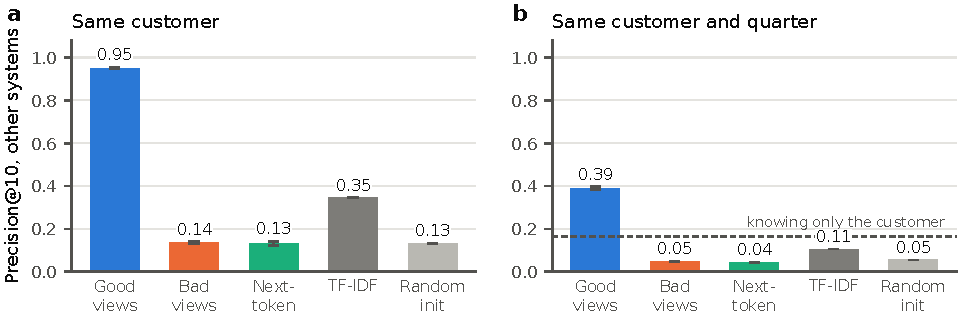
\includegraphics[width=\linewidth]{figures/e1_precision.pdf}
\caption{\textbf{On the training records, only good views put records from different systems about the same situation together.} Precision@10 among neighbours from \emph{other} systems, for the same customer (left) and the same customer and quarter (right). Same text, encoder and budget for the three JEPA objectives; bars show the mean and standard deviation over three seeds. The dashed line is the most a model could reach by recognizing the customer alone.}
\label{fig:e1}
\end{figure}

\begin{table}[t]
\centering
\small
\caption{\textbf{One encoder over all seven systems, measured on the training records} (day~1). Mean $\pm$ standard deviation over three seeds for the JEPA objectives trained from scratch; one seed for the pretrained rows. Cross-system precision@10 for the same customer and the same state (customer and quarter); probe accuracy for the customer, trained on messages and tested on systems of record (M$\to$R) and the reverse; $\rho$ and $R^2$ are fractions of the whitened embedding explained by the state or by the system. The pretrained encoder is all-MiniLM-L6-v2, frozen; its head is trained on good views.}
\label{tab:e1}
\setlength{\tabcolsep}{3.6pt}
\begin{tabular}{lccccccc}
\toprule
& \multicolumn{2}{c}{Precision@10, other systems} & \multicolumn{2}{c}{Customer probe} & & & \\
\cmidrule(lr){2-3}\cmidrule(lr){4-5}
Representation & customer & state & M$\to$R & R$\to$M & $\rho_{\text{state}}$ & $R^2_{\text{state}}$ & $R^2_{\text{system}}$ \\
\midrule
\textcolor{goodblue}{\textbf{Good views}} & \textbf{E1GOODACC} & \textbf{E1GOODST} & \textbf{E1GOODMR} & \textbf{E1GOODRM} & \textbf{E1GOODRHO} & \textbf{E1GOODR2} & E1GOODSYS \\
\textcolor{badorange}{Bad views} & E1BADACC & E1BADST & E1BADMR & E1BADRM & E1BADRHO & E1BADR2 & E1BADSYS \\
\textcolor{ntpaqua}{Next-token} & E1NTPACC & E1NTPST & E1NTPMR & E1NTPRM & E1NTPRHO & E1NTPR2 & E1NTPSYS \\
TF-IDF + LSA & 0.346 & 0.105 & 0.358 & 0.383 & 0.14 & 0.06 & 0.05 \\
Random encoder & 0.132 & 0.055 & 0.188 & 0.150 & 0.17 & 0.05 & 0.04 \\
\addlinespace[2pt]
Pretrained, frozen & PTRAWROW \\
\quad + \textcolor{goodblue}{good-view} head & PTHEADROW \\
\bottomrule
\end{tabular}
\end{table}

Figure~\ref{fig:e1} and Table~\ref{tab:e1} measure how each objective organizes the records it was trained on. With good views, E1GOODPCT of a record's ten nearest neighbours from other systems concern the same customer, against E1BADPCT for bad views and E1NTPPCT for next-token prediction, with the same text and model. TF-IDF reaches 34.6\% and a randomly initialized encoder 13.2\%: with this small encoder, corruption-based views and next-token prediction learn almost nothing about customers. For the state, customer and quarter together, good views reach E1GOODSTPCT against about 4--5\% for the other two objectives; a model that recognized only the customer could reach at most 16.3\%, so the good-view space also separates a customer's quarters. A linear probe trained on messages names the customer of a CRM, support or call record E1GOODMRPCT of the time with good views, and about a quarter of the time with the other objectives. The theorem's scene-explained fraction $\rho$ is about 0.7 for good views and below 0.2 for every other representation trained from scratch, while the system that wrote a record explains about 4\% of the good-view embedding. Figure~\ref{fig:maps} shows the difference: with good views, each customer's records from every system gather in a few tight regions; with the other objectives they are scattered among everyone else's.

The small encoder trained from scratch is a clean control, but it is not what anyone would deploy, and with it bad views and next-token prediction do no better than a random encoder. The last two rows of Table~\ref{tab:e1} repeat the measurement with a pretrained sentence encoder. Out of the box, PTRAWACC of a record's cross-system neighbours concern the same customer, more than TF-IDF. Training only a small head on its frozen outputs with good views raises this to PTHEADACC, more than doubles the cross-family probe from messages to records, and roughly doubles $\rho$. The recipe therefore also improves an encoder that already knows the language. On this company it does not reach the encoder trained from scratch, which can learn the company's own vocabulary (product names, error codes, people); a frozen general-purpose encoder may compress such details away.

These numbers are measured on the records used for training, with the same customer-quarter grouping that defined the positive pairs. They show how well each objective absorbs the links, not how well it generalizes. The next experiment tests generalization.

\begin{figure}[t]
\centering
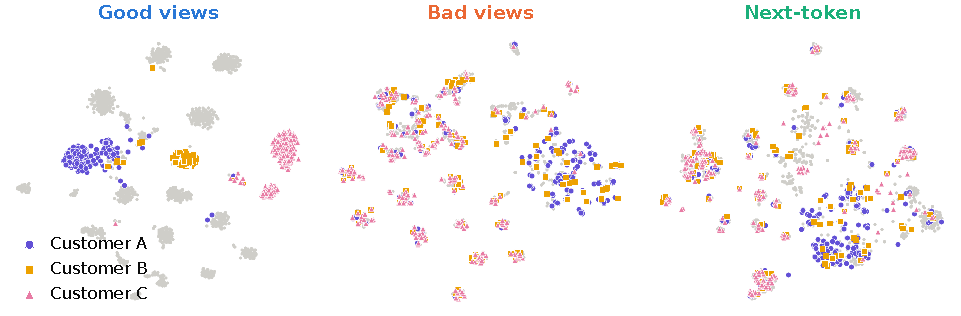
\includegraphics[width=\linewidth]{figures/maps.pdf}
\caption{\textbf{What each objective learns.} Two-dimensional t-SNE maps of the same 3{,}000 training records from all seven systems. Three well-observed customers are highlighted; all other customers are grey. Only good views gather each customer's records, whatever system wrote them.}
\label{fig:maps}
\end{figure}

\subsection{Records whose links were hidden find their place}
\label{sec:heldout}

\begin{table}[t]
\centering
\small
\caption{\textbf{Held-out records.} A quarter of the threads (HONTEST records) were hidden from training: their records were never a view or a prefix. Left: precision@10 among the hidden records, neighbours from other systems. Right: each hidden record is placed at the nearest training state (mean embedding); share placed with the right customer and with the right customer and quarter. One seed.}
\label{tab:heldout}
HOTABLE
\end{table}

We hid a quarter of the threads from training, HONTEST records whose links the model never saw, and trained each objective on the rest. We then placed each hidden record at the training state whose mean embedding is nearest (Table~\ref{tab:heldout}). Good views place HOGOODCUST of the hidden records with the right customer and HOGOODSTATE with the right customer and quarter. TF-IDF places HOTFCUST and HOTFSTATE, bad views HOBADCUST and HOBADSTATE, and next-token prediction HONTPCUST and HONTPSTATE. The pretrained encoder places PTRAWHO with the right customer out of the box, about as many as TF-IDF, and PTHEADHO with a good-view head trained on the same training threads. Knowing each record's customer and choosing that customer's busiest quarter would place HOREFSTATE with the right state, about as many as good views do: on records the model has not seen, the gain is in finding the customer, not in telling that customer's quarters apart; monthly windows change this a little (\secref{sec:time}). Among the hidden records themselves, HOGOODACCPCT of a record's ten nearest neighbours from other systems concern the same customer with good views, against HOTFACCPCT for TF-IDF. Records that carry no link at all, 72\% of this company's records, are in a similar position, although they may differ in kind from linked records (most are chat messages); we cannot score them directly because they have no ground truth.

\subsection{More than names}
\label{sec:mask}

A natural worry is that the encoder merely learns to spot names, as embeddings of earnings calls mostly encode company identity~\citep{yu2024samecompany}. We masked, in every record, the customers' names and their distinctive words, contact names, email addresses, web domains and record identifiers, and retrained the good-view encoder on the masked records (one seed). On the training records, same-customer precision across systems falls from 95\% to MASKGOODPCT, and TF-IDF falls from 35\% to MASKTFPCT (\figref{fig:robust}, right). The company's own employees could still give a customer away, however: an account executive or support engineer who handles a fixed set of accounts is as identifying as a customer's name. We therefore also masked the employees' names, email handles and chat names, in addition to everything above, and retrained again. This mask changes MASKEMPN linked records, against MASKCUSTN for the customer mask alone; most records that name an employee were already changed by it. Same-customer precision is MASKEMPGOODPCT (TF-IDF: MASKEMPTFPCT), and state-level precision is MASKEMPSTPCT, still above the 16.3\% that knowing only the customer would give. Employee names therefore carried almost none of the remaining signal. Roughly half of the customer signal is names and identifiers; the other half comes from what the records say.

\subsection{Wrong links degrade gracefully}
\label{sec:noise}

Real links are imperfect. Tickets get filed under the wrong organization, and duplicate customer records go unmerged. In the theorem, the damage is bounded by how much the wrong links change the positive-pair graph. We attached NOISELOWPCT and NOISEHIGHPCT of linked records to a random wrong state before training (one seed) and evaluated against the true states (\figref{fig:robust}, left). NOISESENTENCE

\begin{figure}[t]
\centering
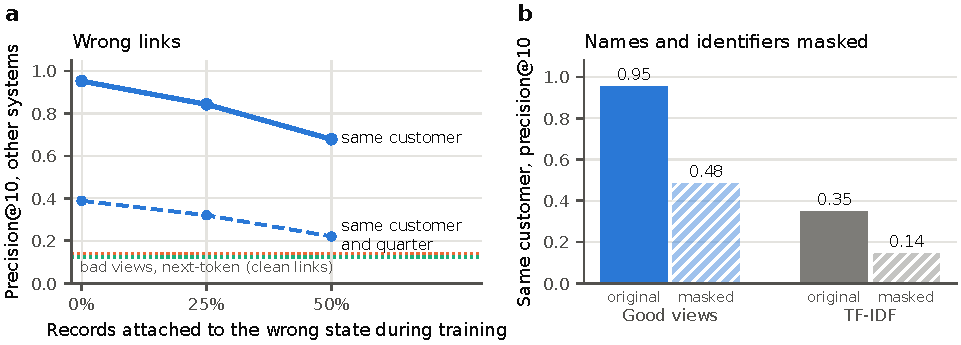
\includegraphics[width=\linewidth]{figures/robustness.pdf}
\caption{\textbf{Robustness, on the training records.} Left: good views trained with a share of records attached to a random wrong state, evaluated against the true states; dashed lines are bad views and next-token prediction with clean links. Right: same-customer precision before and after masking customer names, contacts, domains, email addresses and identifiers from every record.}
\label{fig:robust}
\end{figure}

\subsection{Separately trained encoders can be partly aligned by one rotation}
\label{sec:e2}

\begin{figure}[t]
\centering
\begin{minipage}[t]{0.47\linewidth}
\centering
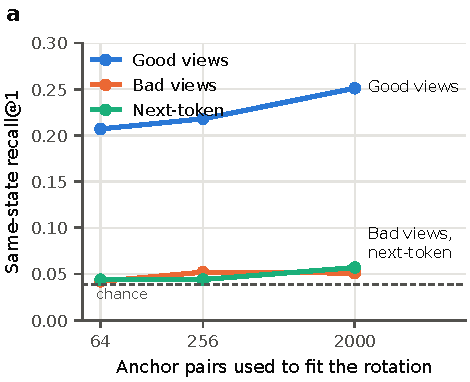
\includegraphics[width=\linewidth]{figures/e2_anchors.pdf}
\caption{\textbf{One rotation partly aligns two separately trained encoders}, one for messages and one for systems of record, but only with good views. Same-state recall@1 of messages retrieving records, on states held out from the rotation fit.}
\label{fig:e2}
\end{minipage}\hfill
\begin{minipage}[t]{0.49\linewidth}
\centering
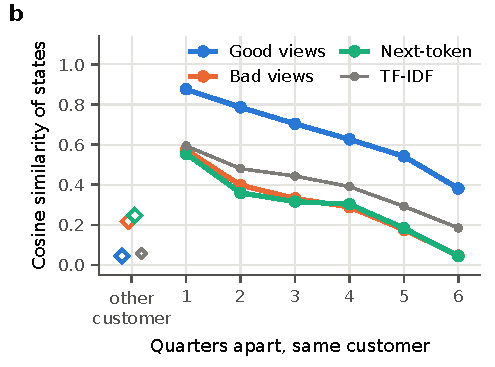
\includegraphics[width=\linewidth]{figures/persistence.pdf}
\caption{\textbf{States persist and drift.} Cosine similarity between centred state vectors of the same customer $k$ quarters apart (lines) and of different customers in the same quarter (diamonds); states with at least five records.}
\label{fig:traj}
\end{minipage}
\end{figure}

We trained one encoder on messages and another on systems of record, with no pair crossing the two, and joined them with one orthogonal map (\figref{fig:e2}). After a rotation fitted on 64 anchor pairs, a message retrieves a record of the same customer and quarter as its top match 20.7\% of the time on states held out from the fit, against 3.8\% by chance; with 2{,}000 anchors, 25.1\%. Same-customer recall@1 is 41--50\% against 14\% by chance. With bad views or next-token prediction no rotation helps: same-state recall stays at 4--6\%, near chance. Before any rotation, the mutual ten-nearest-neighbour agreement between the two spaces is 0.15 with good views and 0.02 with either alternative. The alignment is partial. A message finds a record of the same customer and quarter as its top match only about a fifth of the time; messages and systems of record observe different aspects of a customer's situation, while the theorem's guarantee assumes they observe the same state; and the two encoders share a vocabulary and were trained on the records of the test states, which are held out only from the rotation fit. Still, with good views a single rotation finds shared structure, and with the alternatives it finds none, consistent with the theorem's qualitative prediction.

\subsection{New data and retraining}
\label{sec:e3}

\begin{figure}[t]
\centering
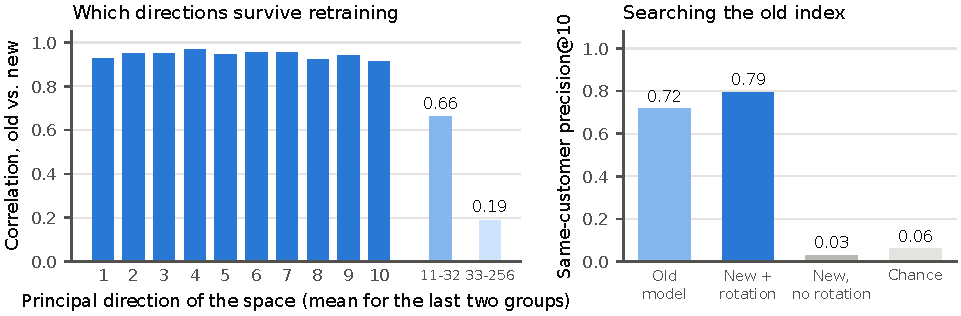
\includegraphics[width=\linewidth]{figures/e3_time.pdf}
\caption{\textbf{Retraining without re-embedding.} Left: correlation between the old model's embeddings and the retrained model's rotated embeddings of the same records, along the old space's principal directions. Right: new-quarter records that neither model was trained on, searched against the old index.}
\label{fig:e3}
\end{figure}

\paragraph{New records.} A customer probe trained on day-1 embeddings assigns 72.6\% of the 7{,}990 records written after training to the right customer with good views, against 41.0\% for next-token prediction and 30.5\% for bad views. The day-1 encoders never saw these records.

\paragraph{New models.} We retrained the good-view encoder on all data through day~2, with the threads of E3BNHIDDEN new records hidden from training, and fitted one rotation and one global scale from the new space to the old on 2{,}000 day-1 records embedded by both. Along the old space's ten leading principal directions, the old and rotated new embeddings correlate at E3BCORR10; from the 33rd direction on, the mean correlation is E3BCORRTAIL (\figref{fig:e3}, left). The leading directions carry most of the variance (the first 16 carry E3BVAR16), so the rotation explains E3BR2 of the variance, but not the low-variance tail. We then used hidden new records, which neither model was trained on, as queries against the old index. Embedded by the retrained model and rotated, they retrieve the same customer with E3BROT precision@10, against E3BUNROT without the rotation and E3BOLD when the old model embeds them (\figref{fig:e3}, right).

Not every measure favours good views. In a second retraining test, scored in a whitened 64-dimensional space that weights every direction equally, a rotation fitted on 256 anchors explains less of a retrained good-view encoder than of a retrained bad-view encoder ($R^2$ of $-0.22$ against $0.28$; mutual ten-nearest-neighbour agreement 0.36 against 0.59). A plausible reading is that bad-view encoders mostly encode surface features of the text, which any retraining reproduces, while the good-view encoder's leading directions, which carry the state, are stable and its tail is not. A rotation registry therefore preserves the part of the space that search relies on, not the whole space.

\paragraph{States persist and drift.} We averaged each customer-quarter's records into a state vector (frozen day-1 encoders, all records through day~2) and compared states (\figref{fig:traj}). With good views, a customer's states in consecutive quarters have a cosine similarity of 0.88, which falls smoothly to 0.38 six quarters apart, while different customers in the same quarter sit at 0.05. With bad views and next-token prediction, consecutive quarters are only 0.55--0.57 alike and different customers 0.22--0.25. In the good-view space a customer's state is persistent yet changes gradually. Whether those changes can be predicted is the question of \secref{sec:time}.

\subsection{Access control, built in}
\label{sec:acl-results}

\begin{table}[t]
\centering
\small
\caption{\textbf{Planted secrets found by readers who may not read them.} Codename search: the share of the ten records returned for a customer's codename that belong to that customer. Secret sentence: the share of the five customers most similar to the planted sentence that are the five canary customers. ``Without'' is the same configuration built from the corpus without the planted secrets. Encoders trained from scratch; one seed.}
\label{tab:acl}
ACLLEAKTABLE
\end{table}

\begin{figure}[t]
\centering
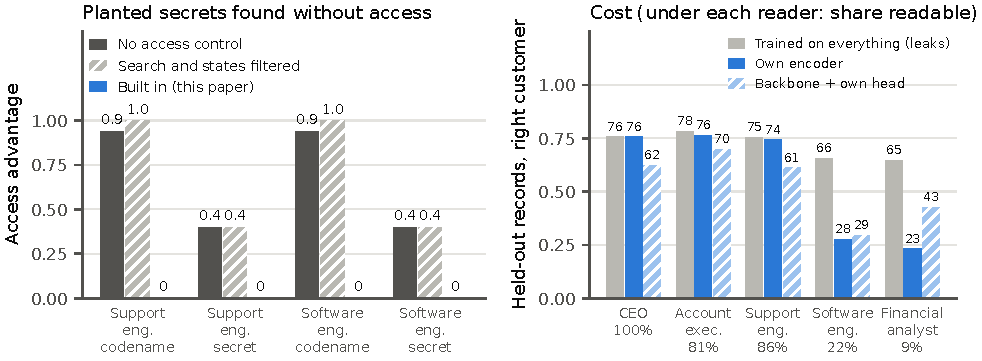
\includegraphics[width=\linewidth]{figures/acl.pdf}
\caption{\textbf{Access control, built in.} Left: how much better two readers without access find the planted secrets (codename search and secret sentence) than they would without the secrets, with no access control, with search and states filtered to readable records, and with access control built in. Right: the share of held-out readable records placed with the right customer by each reader's own non-interfering models, an encoder trained from scratch and a pretrained backbone with a head trained on the reader's records, and by an encoder trained from scratch on everything, which leaks; under each reader, the share of records they may read.}
\label{fig:acl}
\end{figure}

\paragraph{Who may read what.} We gave every record its readers under a role-based policy for the simulated company (Appendix~\ref{app:acl}). The CEO may read ACLVISCEO of the customer-linked records, the support engineer ACLVISSUP, the account executive ACLVISAE, the software engineer ACLVISENG and the financial analyst ACLVISFIN.

\paragraph{Leaks.} We planted secrets in ACLCANARYN CRM and call records of five customers, records that neither the support engineer nor the software engineer may read: a unique codename per customer, and one sentence, the same for all five, saying the customer is expected to churn to a competitor. We then measured what each of the two readers could find, and compared every configuration with the same configuration built without the secrets (Table~\ref{tab:acl}, \figref{fig:acl}, left); the \emph{access advantage} is the share found with the secrets minus the share found without them. Without access control the secrets are in plain view: a codename search returns the right customer's records ACLSUPOPENCODE of the time. Filtering search results and states to readable records, the usual fix, does not stop the leak. The encoder learned the codenames and the sentence from the restricted records and places them next to the right customers' \emph{readable} records. A codename search still returns the right customer's records ACLSUPFILTCODE of the time for the support engineer and ACLENGFILTCODE for the software engineer (ACLSUPFILTNOCODE and ACLENGFILTNOCODE without the secrets). The secret sentence puts ACLSUPFILTSECRET and ACLENGFILTSECRET of the five canary customers among the five most similar customers (ACLSUPFILTNOSECRET and ACLENGFILTNOSECRET without). With access control built in, the readers' encoders never saw the restricted records, and the codenames are not even in their vocabularies: every result is the same with and without the secrets.

\paragraph{Non-interference, checked.} We trained the support engineer's encoder twice, on the corpus with the planted secrets and on the corpus without them. Its training data was byte-for-byte identical, and so was every embedding it produced (largest difference: ACLNIDIFF). The encoder trained on everything changed.

\paragraph{Cost.} What a reader gives up depends on how much they may read (\figref{fig:acl}, right). The CEO reads everything, so nothing changes. The account executive and the support engineer, who may read most records, lose little: their own encoders place held-out readable records with the right customer ACLCOSTAEOWN and ACLCOSTSUPOWN of the time, against ACLCOSTAEOPEN and ACLCOSTSUPOPEN for the encoder trained on everything. The software engineer and the financial analyst, who may read ACLVISENG and ACLVISFIN of the records, lose much more (ACLCOSTENGOWN against ACLCOSTENGOPEN, and ACLCOSTFINOWN against ACLCOSTFINOPEN): their encoders learn from few records, mostly from one or two systems.

\begin{table}[t]
\centering
\small
\caption{\textbf{What a reader can recover without breaking non-interference.} Share of held-out readable records placed with the right customer (nearest readable training state). ``Own encoder'' is trained from scratch on the reader's records; ``backbone'' is the frozen pretrained encoder, which holds no company data; ``backbone + head'' adds a head trained with good views on the reader's records; ``both'' puts the reader's own encoder and their backbone head side by side (run for the two readers who may read least). The last two columns are trained on every record and leak (Table~\ref{tab:acl}). Best non-interfering value per reader in bold. One seed.}
\label{tab:aclrescue}
ACL2TABLE
\end{table}

\paragraph{Recovering accuracy without breaking the guarantee.} The encoder trained on everything is not a fair target: its better placement of a reader's records comes partly from records the reader may not read, which is what non-interference forbids. We tested what a reader can legitimately recover with the two kinds of shared knowledge of \secref{sec:acl} (Table~\ref{tab:aclrescue}). With a frozen pretrained backbone and a good-view head trained on each reader's records, the financial analyst's placement rises from ACLCOSTFINOWN to ACL2FINHEAD; even the backbone with no head places ACL2FINRAW. The software engineer barely gains: ACLCOSTENGOWN with their own encoder, ACL2ENGHEAD with the backbone and a head, and ACL2ENGBOTH with both side by side. For readers who may read most records, the backbone is worse than their own encoder (ACL2CEOHEAD against ACLCOSTCEOOWN for the CEO): a frozen general-purpose encoder with a head is weaker on this company than a small encoder trained on its records, so the backbone can help only where a reader's own data is thin, and it does not always help there. The backbone does not weaken the guarantee. With heads trained on readable records, the access advantage for codenames and for the secret sentence is ACL2SUPBUILTCODEADV and ACL2SUPBUILTSECADV for the support engineer and ACL2ENGBUILTCODEADV and ACL2ENGBUILTSECADV for the software engineer, and each reader's embeddings are identical with and without the secrets (largest difference ACL2SUPNI and ACL2ENGNI). A head trained on every record also leaks through filtered search: the codename advantage is ACL2SUPFILTCODEADV and ACL2ENGFILTCODEADV for the two readers (ACLSUPFILTCODEADVS and ACLENGFILTCODEADVS with the scratch encoder) and the secret-sentence advantage ACL2SUPFILTSECADV and ACL2ENGFILTSECADV (ACLSUPFILTSECADVS and ACLENGFILTSECADVS). The financial analyst may read the CRM records that carry the planted secrets, so the leak test does not apply to that reader; their guarantee, like everyone's, rests on construction.

The second kind of shared knowledge does not help here. Only ACL2PUBRECORDS customer-linked records may be read by every employee (public chat channels and issues). A head trained on them alone places ACL2ENGPUBONLY of the software engineer's held-out records and ACL2FINPUBONLY of the financial analyst's; first trained on them and then fine-tuned on each reader's records for as many steps as a head trained directly, it places ACL2ENGPUB and ACL2FINPUB, against ACL2ENGHEAD and ACL2FINHEAD for the head trained directly on the reader's records. Rotations were not run as an experiment because their effect on accuracy is fixed by geometry: placement by the nearest state centroid under cosine similarity is unchanged by any rotation of the reader's space (a unit test in the repository checks this).

Why do the two readers differ, and where does the loss come from? Almost all of what the software engineer may read (SCOPEENGTOPSHARE) is SCOPEENGTOPSYS, which the backbone alone places poorly (ACL2ENGRAW, against ACL2FINRAW for the financial analyst's records, mostly CRM records): support tickets in this company share templates across customers, and a general-purpose encoder finds little in them that identifies the customer. To separate the number of records a reader may read from their kind, we trained the same scratch encoder on a random sample of records from all systems, as many as each reader may read (SCOPEENGN for the software engineer), and used it to place the reader's held-out records. It places SCOPEENG of the software engineer's records with the right customer (own encoder ACLCOSTENGOWN, everything ACLCOSTENGOPEN) and SCOPEFIN of the financial analyst's (ACLCOSTFINOWN and ACLCOSTFINOPEN). Both matter, and the number matters more: most of the gap to the encoder trained on everything comes from the records a reader may not read at all, and a smaller part from the fact that what they may read comes mostly from one or two systems. Neither part can be recovered from company data the reader may not read. Knowledge from outside the company can make up some of it, as the backbone does for the financial analyst; beyond that, a reader gets more only if the access policy itself gives them more, for example a summary of each customer that everyone may read. That is a decision about access, not about the model.

% -------------------------------------------------------------------------------------------- two channels
\subsection{Two channels: state and detail}
\label{sec:twochannel}

\begin{table}[t]
\centering
\small
\caption{\textbf{Reading facts from customer-quarter states.} Accuracy of linear probes holding out one customer at a time (frozen day-1 encoders, all records through day~2). Two channels are concatenated after each is standardized and scaled to the same total variance; ``system shares'' adds the share of the state's records from each system. Majority class this quarter: tickets 0.57, priority 0.57, call 0.71, stage 0.29; next quarter, 0.49 on average (Appendix~\ref{app:state}). One seed.}
\label{tab:twochannel}
STATE2TABLE
\end{table}

\begin{table}[t]
\centering
\small
\caption{\textbf{Answering the 144 test questions from the store.} Accuracy of the memory reader of Appendix~\ref{app:memory}, closed book (no store) and reading the 16 records retrieved for each question; mean $\pm$ standard deviation over four seeds, and the gain from the store in percentage points. $^{*}$The routed store retrieves with the state channel and reads the detail channel; its questions are embedded as in the detail-only store, so it shares that store's closed-book runs. The four detail-only runs happen to answer the same number of questions (102 of 144), with different answers.}
\label{tab:memory2}
MEM2TABLE
\end{table}

Good-view state vectors are poor at facts about which system recorded what. From a customer-quarter state they read whether a sales call took place CALLGOOD of the time, about the most common answer, while bad-view states read it 97\% of the time; and a store of good-view vectors answered fewer test questions than a store of generic pretrained embeddings (Appendix~\ref{app:memory}). We built the two-channel design this suggests and tested it in both places.

\paragraph{Reading facts from states.} Table~\ref{tab:twochannel} gives the probes of Appendix~\ref{app:state} for single channels and for two channels side by side. A detail channel restores the facts the state channel misses: whether a call took place is read CALLGOOD of the time from good views alone, CALLTWO with the pretrained encoder as the detail channel and CALLGB with bad views. No combination beats the better of its two channels, however. Averaged over the four facts, good views reach NOWGOOD, the pretrained encoder NOWMINI, bad views NOWBAD, and good views with the pretrained encoder side by side NOWTWO. Fact by fact, the concatenated states land between their two channels, usually close to the better one; the deal stage, which good views read best, gets worse when the pretrained channel is added and stays the same with bad views.

\paragraph{Answering questions from the store.} We then built the memory store with four kinds of rows and trained the same reader on each, over four seeds (Table~\ref{tab:memory2}): state vectors only, detail vectors only (the pretrained encoder), both channels concatenated, and both channels routed, retrieving the 16 records nearest the question in the state channel and reading their detail vectors. In every store, the 16 records are those of the question's quarter whose content in the retrieval channel is most similar to the question's (Appendix~\ref{app:memory}). The detail-only store answers MEMMINILM of the questions, the state-only store MEMGOOD, the concatenated store MEMDUAL and the routed store MEMROUTE. Combining the channels does not clearly beat the detail channel alone: paired over the same questions, the concatenated store is MEMPAIRDUALDETAIL ahead of the detail-only store, and the detail-only store MEMPAIRDETAILSTATE ahead of the state-only store. The lead does not come from finding the records: with the customer named in the question, the state-only and detail-only stores retrieve the asked customer's records equally often (MEMRETRGOOD and MEMRETRMINILM of the records retrieved; MEMRETRDUAL for the concatenated store). It comes from reading them, or from how the question is embedded; all four kinds of question (how many tickets, the worst priority, whether a call took place and the deal stage) are about one system's records, which the detail vectors describe more directly. Questions that need the state channel to find the records are absent from this benchmark; the next paragraph builds a version that has them.

\begin{table}[t]
\centering
\small
\caption{\textbf{Questions that come with a record of the customer instead of its name.} ANCHNTEST of the ANCHNALLTEST test questions, each anchored by one record of its customer-quarter from a held-out thread and from a different system than the one that answers it (Appendix~\ref{app:v2}). Records are found among those of the question's quarter: the anchor's 16 nearest neighbours by the finding channel's content alone, the records of the customer whose centroid in the finding channel is nearest to the anchor (placement), or the records of the anchor's own customer-quarter (oracle). The reader then reads the found records' state vectors, detail vectors, or only their system and time codes. Accuracy: mean $\pm$ standard deviation over four seeds, each with its own reader and draw of anchors. Right customer: share of the 16 records found that belong to the anchor's customer. Best store without the oracle in bold, for names kept only.}
\label{tab:anchor}
ANCHORTABLE
\end{table}

\paragraph{When the customer must be found from a record.} Every question so far names its customer, and the detail channel can find the customer's records by name. We built a version in which it cannot (Table~\ref{tab:anchor}; Appendix~\ref{app:v2}). The question no longer names the customer; it comes instead with one record of the customer, its \emph{anchor}, as if asked by someone holding that record: a support ticket in hand, was there a sales call with this customer this quarter? The anchor comes from a thread hidden from the state encoder's training, and from the reader's pre-training, and from a different system than the one that answers the question, so the reader must find the customer's other records across systems from one record without its link. We ran this twice, with the names of customers and employees and all identifiers masked in every stored record and question, and with them kept. A store finds 16 records of the question's quarter for the reader in one of three ways: the anchor's nearest neighbours by the content of one channel; placement, which takes the records of the customer whose centroid in that channel is nearest to the anchor (\secref{sec:heldout} places records at customer-quarter centroids; here the quarter comes from the question); or, as an oracle, the records of the anchor's own customer-quarter.

\textbf{With names kept, finding the records with the state channel helps most.} Placement with the state channel finds the right customer for ANCHPPLACESTATECUST of the records read and answers ANCHPPLACESTATEACC of the questions; placement with the pretrained encoder finds it for ANCHPPLACEDETAILCUST and answers ANCHPPLACEDETAILACC. Paired over the same questions and anchors, the difference is ANCHPPAIRSTATEDETAIL. Nearest neighbours point the same way but less clearly: the state channel's neighbours are from the right customer ANCHPSTATECUST of the time and the detail channel's ANCHPDETAILCUST, yet read through the detail channel they answer ANCHPROUTEDACC against ANCHPDETAILACC for the detail channel's own neighbours. Neighbours are records like the anchor; placement reads a sample of the whole situation, which more often contains a record of the system that answers the question (ANCHPPLACESTATEUSE of the records read are such records from the right customer-quarter, against ANCHPROUTEDUSE for the state channel's neighbours and ANCHPDETAILUSE for the detail channel's). Placing with both channels concatenated does about as well as the state channel alone (ANCHPPLACECONCATACC). The best store without the oracle comes within ANCHPGAPORACLE points of the oracle (ANCHPLINKACC) and well above no store (ANCHPCLOSEDACC); paired with no store, placement with the state channel gains ANCHPPAIRSTATECLOSED.

\textbf{With every name masked, the customer can rarely be found from one record.} The state channel still places held-out masked records with the right customer more often than the detail channel (ANCHMHOSTATE against ANCHMHODETAIL). Its nearest neighbours, read through the detail channel, help a little: they answer ANCHMROUTEDACC against ANCHMCLOSEDACC with no store, a paired gain of ANCHMPAIRROUTEDCLOSED. Placement does not: it answers ANCHMPLACESTATEACC, a paired gain of ANCHMPAIRSTATECLOSED. The oracle answers ANCHMLINKACC.

\textbf{Which vectors the reader reads matters much less.} Given the oracle's records, reading state vectors answers ANCHMLINKSTATEACC of the questions with names masked and reading detail vectors ANCHMLINKACC (ANCHPLINKSTATEACC and ANCHPLINKACC with names kept). Reading only each record's system and time codes, with no content at all, answers ANCHMLINKPROVACC and ANCHPLINKPROVACC. For questions about how many tickets there were or whether a call took place, the provenance of the right records carries most of the answer.

\paragraph{What the two channels are for.} The channels do different jobs. The state channel finds the situation: it places held-out records with the right customer HOGOODCUST of the time against PTRAWHO for the pretrained encoder (Table~\ref{tab:heldout}), and in a memory, finding a question's records through it is what helps most when the question comes with a record of the customer rather than a name, at least when names are kept in the records. The detail channel finds records by what they literally say, including names, and, as \secref{sec:primitives} shows, finds other customers in similar trouble, which the state channel does not. Once the right records are found, their provenance carries much of what counting questions need. Keeping both channels is useful because a world model needs both abilities; blending them in one vector does about as well as the better of the two for finding and no better for answering. What a memory needs is to find a query's records through the state space, or by name when it has one, before reading them.

% -------------------------------------------------------------------------------------------- time
\subsection{Finer time windows and dynamics}
\label{sec:time}

\begin{table}[t]
\centering
\small
\caption{\textbf{Quarters and months.} Held-out records (the threads of Table~\ref{tab:heldout}) placed at the nearest training state, with states defined by quarter or by month. Each good-view encoder is trained with the states it is evaluated on. One seed.}
\label{tab:months}
MONTABLE
\end{table}

\begin{table}[t]
\centering
\small
\caption{\textbf{Month-to-month dynamics} (TIMESTATES customer-month states, TIMETRANS transitions, frozen day-1 encoders, all records through day~2). Next-month facts: mean accuracy of linear probes predicting next month's four facts from this month's state, holding out one customer at a time. Dynamics, in the 32 leading principal components of the standardized states, also holding out one customer at a time: cosine between this month's and next month's state, and the squared error of three predictors relative to predicting no change (negative is better): a linear map from the state to its change (ridge regression with $\alpha = 10$, or with $\alpha$ chosen by nested leave-one-customer-out validation), and shrinking the state toward the mean by one fitted factor. One seed.}
\label{tab:time}
TIMETABLE
\end{table}

With quarters as windows the company has 180 states on day~1 and, with all records through day~2, 202 states and 165 quarter-to-quarter transitions, too few to learn how states change. Re-slicing the same records by calendar month gives MONSTATES states on day~1 and, with all records through day~2, TIMESTATES states and TIMETRANS month-to-month transitions; ISO weeks give PRIMWEEKS customer-weeks with enough records to compare (\secref{sec:primitives}).

\paragraph{Telling months apart.} We trained a good-view encoder with customer-month states on the training threads of \secref{sec:heldout} and placed the hidden records (Table~\ref{tab:months}). It places MONGOODCUST with the right customer and MONGOODMONTH with the right customer and month, against MONREF for knowing the customer and choosing its busiest month. With quarters, good views did no better than knowing the customer and choosing its busiest quarter; with months, they do somewhat better, so finer windows let the model use some of the time information in the text. The pretrained encoder, with or without a good-view head, finds the right month less often than the busiest-month reference (MONRAWMONTH and MONHEADMONTH).

\paragraph{Forecasting and linear dynamics.} Month states do not predict the next month (Table~\ref{tab:time}). Probes holding out one customer at a time predict next month's facts no better than the most common answer (TIMEMAJ on average, against FCGOODMONTH for good-view month states, FCBAD for bad views and FCTWO for two channels), far below copying this month's true facts (TIMEORACLE). We also fitted the simplest dynamics model, a linear map from a month's state to its change into the next month (ridge regression), and compared it with predicting no change and with shrinking the state toward the average state by one fitted factor, itself a linear predictor. With a fixed, weak regularization ($\alpha = 10$) the map overfits: in the good-view space it increases the squared error by DYNGOODERR relative to predicting no change. With the regularization chosen by nested leave-one-customer-out validation it reduces the error in every space (by TUNEDRANGE), but never by more than TUNEDMAXGAIN points beyond what the single shrinkage factor achieves, and in TUNEDNWORSE of the six spaces by no more at all. The bad-view and pretrained spaces are noisy from month to month, so the best linear guess moves the current state about halfway toward the average (shrinkage factors SHRINKKBAD and SHRINKKMINI); good-view month states are smoother (factor SHRINKKGOOD, cosine DYNGOODCOS between consecutive months). Almost everything a linear model learns here is mean reversion: two to three times as many transitions are not enough to learn how a customer's situation moves in this data. This predictor has no actions; \secref{sec:decisions} adds the company's.

% -------------------------------------------------------------------------------------------- primitives
\subsection{Operational primitives: drift, misalignment and similar situations}
\label{sec:primitives}

\begin{table}[t]
\centering
\small
\caption{\textbf{Operational primitives against Era's ground truth} (all records through day~2, frozen day-1 encoders). Drift: AUROC of the weekly drift score for weeks with an urgent or high-priority ticket or a deal-stage change, and for the week before one. Misalignment: AUROC of the distance between a customer's sales and support records for months with an urgent or high-priority ticket during an open deal. Similar situations: share of the five most similar states of \emph{other} customers that share a quarter's situation (ticket count and deal stage), among all of them or only those in other quarters, and, for customers in trouble, the share of the five that are also in trouble. One seed.}
\label{tab:primitives}
PRIMTABLE
\end{table}

Section~\ref{sec:what} promised that a shared state space turns operational questions into geometry. We tested three such questions against Era's ground truth (Table~\ref{tab:primitives}; details in Appendix~\ref{app:v2}).

\paragraph{Is something off? Drift.} For every customer and ISO week with at least three records, we computed a state vector and scored the week by its cosine distance from the mean of the customer's previous one to four weekly states within eight weeks (PRIMWEEKS customer-weeks). If the state moves when the situation does, high scores should mark the PRIMEVENTS weeks with an escalation (a new urgent or high-priority ticket) or a change of deal stage, or the weeks just before them. They do not, beyond noise: the AUROC is DRIFTRANGE for every representation, within about two standard errors of chance ($0.50 \pm$ DRIFTSE2), against DRIFTVOL for a score that uses only the change in the number of records.

\paragraph{Is something off? Misalignment between teams.} For every customer-month with at least two sales records (CRM and calls) and two support records (tickets and issues), we computed the cosine distance between the sales view and the support view of the customer (MISWIN customer-months). If the two teams' records drift apart when a customer is at risk, the distance should be larger in the MISRISK months with an urgent or high-priority ticket during an open deal. It is not: the AUROC is MISRANGE, within two standard errors of chance ($\pm$MISSE2 with so few months at risk).

\paragraph{What is this like? Similar situations across customers.} For every customer-quarter state with at least five records (SITSTATES states), we retrieved the five most similar states of \emph{other} customers and checked whether they share its situation, defined from the ground truth as the number of tickets (four buckets) and the deal stage (open, won, lost or none). Here every representation does better than chance: SITGOOD of the retrieved states share the situation with good views and SITBAD with bad views, against SITCHANCE by chance. This is not just the calendar. Restricted to other customers' states in other quarters, precision is SITOTHERQGOOD against SITOTHERQCHANCE by chance, and picking other customers in the same quarter would give SITSAMEQ. For customers in trouble, quarters with an urgent or high-priority ticket during an open deal (TROUBLEN states), the channels differ sharply. Among the five most similar states of other customers, TROUBLEBAD are also in trouble with bad views and TROUBLEMINI with the pretrained encoder, against a base rate of TROUBLEBASE, but only TROUBLEGOOD with good views and TROUBLETWO with the two channels concatenated. Trouble, defined this way, rests on facts about particular systems' records (ticket priorities and deal stages), the kind of fact the detail channel keeps and the state channel discards.

Two of the three primitives fail on this data. The third works with every representation, and for customers in trouble only with the channels that keep detail. We see three possible reasons for the failures and cannot separate them here: Era may generate escalations without precursors in the text of other systems; weekly and monthly states average few records and are noisy; and none of the encoders was trained to register change, since good views make the state stable by design and the other objectives are not trained on time at all. A world model that answers ``is something off?'' will probably need a predictor trained for it, on more transitions than one simulated company provides, rather than distances in a space trained for something else.

% -------------------------------------------------------------------------------------------- decisions
\subsection{Decisions: what the company did, and what followed}
\label{sec:decisions}

\begin{table}[t]
\centering
\small
\caption{\textbf{Decisions and dynamics} (ACTTRANS month-to-month transitions of the 21 customers in the day-2 corpus, frozen day-1 encoders, one run). Top: squared error of next month's state, in the 32 leading principal components, relative to predicting no change (negative is better), holding out one customer at a time, with the ridge strength chosen by nested validation. ``State'' predicts the change from this month's state alone; the next two columns add this month's six actions, as recorded and shuffled across months; the last two add next month's actions, which are recorded in next month's state itself, and next month's mix of systems, the share of its records that each system wrote. Bottom: next month's outcomes predicted from the 16 leading components of this month's state, with and without this month's actions, holding out one customer at a time; $^{*}$, the 95\% interval of the gain over customers excludes zero. ``Actions alone'' is a model of the six indicators, held out the same way; the last row scores the support-reply indicator itself.}
\label{tab:actions}
ACTDYNTABLE
\end{table}

\begin{table}[t]
\centering
\small
\caption{\textbf{Simulating a decision for customers in trouble} (SIMTROUBLE customer-months with an urgent or high-priority ticket during an open deal). ``Intervene'': a sales call or an engineering escalation in the month of trouble. Each row estimates what follows the two decisions: the outcomes observed in the months in trouble; those that followed the most similar states of other customers, up to SIMK in which the company intervened and SIMK in which it did not among the SIMPOOL nearest (case-based simulation, in four state spaces); those of all other customers' months, without matching; and a logistic outcome model of the state and the decision. Differences in percentage points, computed before rounding, with 95\% intervals in brackets from resampling customers, repeating the neighbour search and refitting the outcome model. Observational: what followed each decision, not its effect.}
\label{tab:simulate}
SIMTABLE
\end{table}

Section~\ref{sec:what} defines the predictor of a world model as action-conditioned, $s_{e,t+1} \approx h(s_{e,t}, a_t)$; the dynamics of \secref{sec:time} had no actions. The records say what the company did. For each customer and month we read six actions from the records and Era's ground truth (Appendix~\ref{app:v2}): a sales call held (ACTSHARECALL of customer-months), a leader, the CEO or the head of engineering, writing to or about the customer (ACTSHARELEADER), a CRM task logged (ACTSHARECRMTASK), an engineering escalation, a Jira issue opened for the customer (ACTSHAREENGESC), support agents replying on the customer's tickets (ACTSHARESUPPORT), and employees writing on the customer's email threads (ACTSHAREOUTBOUND). Outcomes come from the ground truth: a deal advancing or being won (in ACTPROGRESSRATE of months) and an urgent or high-priority ticket (ACTESCRATE). Actions and outcomes travel together: a deal advanced in ACTCALLPROGNEXT of the months with a sales call and ACTNOCALLPROGNEXT of the months without one. Every comparison below is observational; the company's actions were not randomized.

\paragraph{Action-conditioned dynamics.} We added the six actions to the linear predictor of \secref{sec:time} (Table~\ref{tab:actions}, top). This month's actions do not help predict next month's state. Relative to the state alone, they change the error by ACTLAGRANGE of the state-only error across the four representations (positive is worse; good views ACTGOODLAG, 95\% interval ACTGOODLAGCI); the same actions shuffled across months cost ACTSHUFRANGE, and this month's mix of systems changes the error by ACTMIXRANGE. In the good-view and bad-view spaces, one reason is that the state already holds the actions: from the 16 leading components of this month's state, a logistic regression holding out one customer at a time predicts each of the six with AUROC ACTFROMSTATEGOOD and ACTFROMSTATEBAD. In the pretrained and two-channel spaces they are harder to read (ACTFROMSTATEMINI and ACTFROMSTATETWO) and still add nothing, so redundancy is not the whole explanation. Next month's actions do help, lowering the error by a further ACTNEXTRANGE of the state-only error (good views ACTGOODNEXT, interval ACTGOODNEXTCI). They are, however, also a description of next month's records: a Jira record is an engineering escalation, and each of the other actions is a kind of record of one system. Next month's mix of systems, the share of next month's records that each system wrote, lowers the error by about as much on average (ACTNEXTMIXRANGE), though unevenly across customers (ACTNEXTMIXSIG), and with the mix in the model, next month's actions lower it by a further ACTNEXTBEYONDRANGE (ACTNEXTBEYONDSIG). Much of what next month's actions add is what they say about the records next month's state is built from.

\paragraph{Outcomes.} For what happens to the customer, this month's actions do add signal, but mostly through the persistence of tickets (Table~\ref{tab:actions}, bottom). From this month's state, a deal advancing next month is predicted with AUROC ACTAUCPROGSTATERANGE across the four representations and an urgent ticket with ACTAUCESCSTATERANGE. Adding this month's actions changes these by ACTAUCPROGDIFFRANGE and ACTAUCESCDIFFRANGE; the interval excludes zero in ACTAUCPROGNSIG of the four representations for deals and in ACTAUCESCNSIG for urgent tickets, and the gain is largest where the state is weakest. The signal sits in support replies: adding only them to the state gives the same AUROC as adding all six actions (differences ACTSUPVSALLRANGE, ACTSUPVSALLSIG), and the reply indicator by itself ranks next month's urgent tickets with AUROC ACTSUPONLYESC. A support reply marks a month with a ticket (ACTSUPTICKET of months with a ticket have one, ACTSUPNOTICKET of months without), and the indicator of any ticket this month ranks next month's urgent tickets as well (AUROC ACTTICKETAUC). Customers with tickets keep having them, and the reply mostly marks that persistence rather than the effect of a decision.

\paragraph{Around single actions.} At a finer scale, we compared the good-view state in the 14 days before and after an action with the same customer's state around a time with no action of that kind within 14 days, leaving all records of the action's kind out of both windows. The actions are the EVCALLN sales calls (at EVCALLCUST customers), EVENGESCN engineering escalations (EVENGESCCUST customers) and EVLEADERN first leader messages after a quiet fortnight (EVLEADERCUST customers) that have at least two other records of the customer on each side. The state moves more around engineering escalations than at matched times: 1 $-$ cosine is EVENGESCSHIFT against EVENGESCMATCH, a difference of EVENGESCDIFF. Their windows hold more records, though (a median of EVENGESCRECEV before the event against EVENGESCRECMATCH), and with each window's record count accounted for, the difference is EVENGESCADJ. Around sales calls it is EVCALLADJ, and around leaders' messages EVLEADERADJ, from only EVLEADERMATCHN matched times, because leaders write about most customers often. Knowing which action was taken does not help predict where the state goes either: across EVPAIRS pairs of windows, it changes the error of a linear predictor by EVPRED.

\paragraph{Simulating a decision.} For the SIMTROUBLE customer-months in trouble, an urgent or high-priority ticket during an open deal, we asked the question a world model of a company is for: what follows if the company intervenes, with a sales call or an engineering escalation, and what if it does not (Table~\ref{tab:simulate})? The months come from SIMCUST customers, SIMMAXCUST of them from one. The machinery works: the state space retrieves similar situations of other customers, splits them by what the company did, and returns what followed. The answers cannot be taken as effects, and the data show why. First, the logs barely contain the alternative: the company intervened in SIMINTERV of the SIMTROUBLE months and held back in SIMNOT. Second, decisions follow situations that the state does not fully capture. Whether the company intervened in a month can be predicted from the month's state (AUROC SIMPROPRANGE across the four representations, holding out one customer at a time), yet among the most similar states of other customers, those in which the company intervened were themselves in trouble SIMBALTROUBLEONR of the time and had an urgent ticket SIMBALESCONR of the time across the four spaces, against SIMBALTROUBLEOFFR and SIMBALESCOFFR for those in which it did not (in the good-view space, SIMBALTROUBLEON and SIMBALESCON against SIMBALTROUBLEOFF and SIMBALESCOFF). The case-based comparison therefore sets troubled months against calm ones, and intervening appears to be followed by more urgent tickets (SIMESCCASE points, interval SIMESCCASECI), which is what one would see if calls and escalations are made when problems are severe, whatever their effect. The estimates also move with the space used to find similar states (SIMPROGCASERANGE points for deals and SIMESCCASERANGE for urgent tickets, with SIMCASENZERO of the eight intervals including zero), and the outcome model, which takes the decision as an input, attributes little to it (SIMPROGMODEL and SIMESCMODEL points). Within the months in trouble, the first call or escalation came before the month's first urgent ticket in SIMBEFORE and after it in SIMAFTER, so a monthly action indicator mixes responses to a ticket with actions taken before it.

The decision layer of an operational world model can thus be built on the state space from the company's own records, without new data: actions, action-conditioned transitions, event windows and decision simulation. On one company's logs it learns little about what decisions do. This month's actions add nothing to next month's state, and in the link-trained space the state already encodes most of them; next month's actions help mostly by describing the records next month's state is built from; no single action moves the state detectably more than matched times once record counts are accounted for; and the company intervened in situations unlike those in which it held back, in ways that matching on the state did not remove in any of the four spaces. Learning from decisions will need actions whose assignment is known: decisions logged with their reasons, deliberately varied, or replayed in a simulator that can run the same situation with a different decision.

% ============================================================================================ 7
\section{Why this matters: from records to a model of the company}
\label{sec:why}

Most enterprise AI today is retrieval: given a question, find documents, read them, answer and forget. Every question pays the full cost of rebuilding the situation, and two questions about the same customer may rebuild it differently. A world model inverts this. The organization's state is maintained continuously as records arrive, and questions are answered from the state. The path from records to such a model has four steps, each useful on its own and each making the next possible: (1) a shared state space learned from the links an organization already keeps, the subject of this paper; (2) a memory that stores both the state and the detail of every record and serves each question from the channel suited to it; (3) a predictor of how states change, trained on the organization's own history of states, decisions and outcomes; and (4) planning, in which people and agents try decisions against the predictor before making them. Four properties make the first step practical, and the experiments above speak to each, with the caveats noted.
\begin{itemize}
\item \textbf{No annotation.} The training signal is the link structure the organization's systems already keep (\secref{sec:e1}, \secref{sec:heldout}). Nobody labels anything, wrong links blur the space instead of breaking it (\secref{sec:noise}), and the same signal improves an off-the-shelf pretrained encoder (\secref{sec:e1}).
\item \textbf{Records without links find their place.} Records whose links were hidden during training are placed with the right customer by what they say (\secref{sec:heldout}), and masking the names of customers and employees in the training records shows that the space is built from more than names (\secref{sec:mask}).
\item \textbf{Every system, one space.} Encoders trained separately for different systems can be partly aligned by one rotation fitted on matched records (\secref{sec:e2}). A new tool, or an acquired company's chat, could join this way without retraining everything; we have not tested that directly.
\item \textbf{Memory that survives upgrades.} One rotation lets a retrained encoder search the old index (\secref{sec:e3}). If that holds across many upgrades, which we have not tested, an organization's memory can compound across model versions instead of being rebuilt with each one.
\end{itemize}
\paragraph{A division of labor.} The experiments draw sharper lines between the parts of a world model than we expected. The state space, the first part, can be learned from links alone, places records that carry no link, can be shared across encoders and versions through rotations, and can carry access control. Memory, the second part, should find through the state space and read from the store. When a question names its customer, the records can be found by name; when it comes with a record instead, finding the customer's records through the state space is what helps, clearly when the record is placed in the space and less clearly through its neighbours, and the store's job is then to supply what those records say and where they came from (\secref{sec:twochannel}). The third part, a predictor, did not emerge here from a space trained for static similarity: with 2.4 times as many transitions, linear models learn little beyond mean reversion, and drift and misalignment scores are at chance (\secref{sec:time}, \secref{sec:primitives}). Conditioning it on the company's logged actions does not change that, and simulating decisions from the logs returns the situations in which the company acted rather than the effect of acting (\secref{sec:decisions}). We expect a predictor to need transitions from many companies and actions whose assignment is known: logged with their reasons, deliberately varied, or replayed in a simulator. These lines are drawn on one simulated company and may move with more data.

\paragraph{Cheap enough to retrain often.}
Every encoder and head we timed trains in TRAINMINLO--TRAINMINHI minutes on a CPU, without a GPU: the state encoder from scratch, each reader's encoder, the head on the pretrained backbone and the month encoder (each reader's head on the backbone, which we did not time, is the same head trained on fewer records). The memory reader, pre-training included, took at most MEMREADERMIN minutes. At this scale a company could retrain its state space, and the model of every access scope, daily or whenever an access rule changes, where adapting a large language model to the same data would typically need GPUs. That matters for corporate AI, where the data change daily and every change must reach only the people allowed to see it. Whether training stays this cheap for a company with millions of records is untested.

\paragraph{Access control is part of the model.}
Enterprise systems took decades to encode who may see what. A world model that flattens those rules into one shared representation undoes that work, however carefully its search results are filtered: our experiments show restricted content leaking through the encoder's weights even when every search result and every state shown is computed from readable records (\secref{sec:acl-results}). Aggregation is a third path that a filtered index does not close; we argue it from the construction of states rather than measure it separately. Building the three controls into the model instead keeps each person's view complete within their rights and empty outside them, with a guarantee that holds by construction. It also makes the model easier to trust and to audit: deleting a record, and retraining the encoders of the scopes that could read it, removes its influence from every view that could see it, and from no other. The guarantee has a price for people who may read little, and knowledge without company data repays it only partly. What a support ticket means is learned largely from the emails, calls and CRM records around it, and a reader who may not read those cannot have that knowledge from the model either (\secref{sec:acl-results}).

\paragraph{What changes for a company.}
When people and AI agents read the same state, hand-offs, onboarding and reviews start from the state instead of from a search. Because the state space is shared, what the organization knows accumulates in one place instead of in each person's head, and it stays usable when people leave. Whether coordination becomes measurable, for instance whether two teams whose records about the same customer drift apart are misaligned before anyone notices, is a hypothesis we could not confirm on this data (\secref{sec:primitives}).

\paragraph{Toward dynamics.}
A state space is the first half of a world model. The second half is a predictor over it: given a customer's state this quarter and an action, such as a discount, an escalation or a new owner, what is the likely next state? Predictors trained in a learned latent space are how world models are built for video and robotics~\citep{lecun2022path,hafner2020dreamer}. In an organization, the training data for such a predictor is the history of states, decisions and outcomes that the company already records. Our results show that 165 quarterly or 398 monthly transitions from one company are not enough: a linear predictor learns little beyond mean reversion; many companies, explicit actions, and objectives that reward predicting change rather than holding the state still will be needed. Our attempt to condition the predictor on the company's own actions (\secref{sec:decisions}) suggests what such training data must contain: decisions whose assignment is known, because they were logged with their reasons, varied on purpose, or replayed in a simulator. With a predictor, a company can ask ``what happens if'' before acting, and agents can plan against a model of the organization instead of against documents.

\paragraph{Personal world models.}
The same recipe applies to one person. Their email, calendar, messages and documents are different observations of their own projects and relationships, linked by people, threads and time.

\paragraph{Why we expect every company to have an operational world model.}
Every company already has a world model: it is distributed across the heads of its people, partial, inconsistent and lost when they leave. Making it explicit changes three things. People and agents can \emph{understand} how the company is functioning from one shared, permission-respecting state instead of reassembling it from documents. They can \emph{learn} on it the way a person learns a company, from its own history of situations, decisions and outcomes, with a predictor over the state space as the learning substrate. And they can \emph{improve} the company by trying a decision against the model before making it, and by seeing where the company's actual trajectory departs from the one it planned. The state space and the access control studied here are the foundation those three uses share; the predictor that the second and third uses need is the open problem our negative results point to.

% ============================================================================================ 8
\section{Related work}
\label{sec:related}

\paragraph{Linked records as positives.} Treating records that share a link as positive pairs is established: citations~\citep{cohan2020specter}, authors and venues~\citep{zhang2022metadata}, product identifiers~\citep{peeters2022supervised}, foreign keys in relational databases~\citep{peleska2025relational}, one bank client's transactions, locations and support calls~\citep{mollaev2025banking}, one patient's codes and notes~\citep{cai2024ehr} and, in industry, per-company embedding models fine-tuned on document links, co-access and chat threads.\footnote{\url{https://jxnl.co/writing/2025/03/06/fine-tuning-embedding-models-for-enterprise-rag-lessons-from-glean/}} The closest is the multimodal banking work, which trains one encoder per modality jointly with a CLIP-style objective~\citep{radford2021clip}. We differ in defining states by entity \emph{and} time window across a company's systems, training per-system encoders separately and joining them by a rotation, and testing the predictions of the Platonic Representation Theorem against bad-view and next-token controls. Where the industrial practice fine-tunes a pretrained sentence encoder~\citep{reimers2019sbert}, we also train only a head on a frozen one, which keeps the backbone free of company data and therefore shareable across access scopes.

\paragraph{JEPAs for text.} LLM-JEPA applies a JEPA loss to curated pairs of text and code that describe the same thing~\citep{huang2025llmjepa}, and \citet{zuo2026asymmetric} apply JEPA with SIGReg to sections of a scientific paper. Our views come from organizational links, and our encoder is trained from scratch on one company.

\paragraph{Convergence and alignment of representations.} Beyond the Platonic hypothesis and theorem~\citep{huh2024platonic,balestriero2026platonic}, anchors and orthogonal maps join independently trained latent spaces~\citep{moschella2023relative,maiorca2023latent} and data silos~\citep{nosaka2024collaboration}, and orthogonal Procrustes has aligned word embeddings across decades~\citep{hamilton2016diachronic}. Theory relates self-supervised representations to the spectrum of the positive-pair graph~\citep{haochen2021spectral} and to the content that views share~\citep{vonkugelgen2021content}.

\paragraph{Compatible embeddings across model updates.} Backward-compatible training makes a new model's embeddings comparable with an old index~\citep{shen2020bct}; fitted Procrustes maps or affine adapters do so after training~\citep{maystre2025procrustes,vejendla2025drift}. Our rotation registry is an instance of the latter; for good-view encoders it preserves the leading directions of the space but not the tail.

\paragraph{Access control in machine learning.} Information flow control for machine learning trains one expert module per security domain and combines only the experts a user may access, which gives non-interference for language models~\citep{tiwari2024ifc}. Permissioned LLMs attach parameter-efficient adapters to security domains and measure leakage with an access-advantage metric~\citep{jayaraman2025permissioned}, and a position paper argues that enterprise models must be trained, and retrieve, only on content that every participant in an interaction may access~\citep{bhatt2025participant}. Permission-aware retrieval, which filters search results by the reader's rights, is standard industry practice. We bring these ideas to a learned world model of an organization, where a third leak path appears, aggregation of records into states, and we measure what readers who may read little can recover from shared knowledge without breaking non-interference.

\paragraph{Memory for language models.} Memorilla compresses a document collection into a few query-dependent memory tokens for a frozen model~\citep{fallahpour2026memorilla}, and xRAG compresses a retrieved document into one token~\citep{cheng2024xrag}.

\paragraph{Simulated organizations and enterprise world models.} Era by Eon~\citep{gruenbaum2026era}, OrgForge~\citep{flynt2026orgforge}, TheAgentCompany~\citep{xu2024theagentcompany} and CRMArena~\citep{huang2024crmarena} simulate companies to evaluate agents; we use one to learn representations. \citet{nair2026enterprise} study learned world models of enterprise systems as predictors of state transitions and find that they falter when a deployment's configuration changes. Organizational memory has a long history in management research~\citep{walsh1991organizational}, and object-centric process mining relates events to the business objects they touch~\citep{vanderaalst2019object}. For individuals, general user models are built from a person's computer use and kept as text statements~\citep{shaikh2025gum}.

% ============================================================================================ 9
\section{Limitations}
\label{sec:limits}

\begin{itemize}
\item \textbf{One simulated company.} All results come from one Era company with 21 active customers. Era's text is cleaner and more regular than real company text, and its systems agree by construction. Replication on more simulated companies, and on real data, is the most important next step. Several negative results (drift, misalignment, forecasting) may reflect how Era generates events rather than what a state space can do: if escalations have no precursors in the text of other systems, no representation of that text can anticipate them.
\item \textbf{Weak supervision, evaluated partly on itself.} Links are not annotations, but they are supervision: the positive pairs come from the same customer-quarter grouping that most of our metrics score. Results on training records (\secref{sec:e1}, \secref{sec:mask}, \secref{sec:noise}) are therefore upper bounds; the held-out test (\secref{sec:heldout}) is the fairer measure.
\item \textbf{Weak alternatives from scratch.} With our small encoder, corruption-based views and next-token prediction learn little about customers on training records (no better than a random encoder there). The pretrained encoder is a stronger baseline, and good views improve it too, but we tested only one small, frozen backbone; fine-tuning a larger encoder end to end may behave differently.
\item \textbf{Seeds.} The main comparison uses three seeds and the memory reader four; the held-out, alignment, time, masking, noise, pretrained, access-control, primitive and decision experiments use one.
\item \textbf{Partial alignment.} Separately trained encoders agree on the leading directions, not on the tail, and messages and systems of record share only part of the state.
\item \textbf{A narrow, partly constructed question benchmark.} The 144 test questions ask only about counts and categories within one system's records. The anchored version is constructed to need the state channel: its anchors come from held-out threads and from systems other than the one that answers the question, retrieval takes the quarter from the question, and questions without such an anchor are dropped (ANCHNTEST of ANCHNALLTEST test questions remain). Its four seeds vary the reader and the anchors but not the state encoder, which is one run. Questions that need several systems' records at once, or that come with several records of the customer, remain untested.
\item \textbf{No dynamics yet.} Neither forecasts nor a linear predictor beat simple baselines with quarterly or monthly windows (\secref{sec:time}), conditioning the predictor on logged actions does not change that (\secref{sec:decisions}), and drift and misalignment scores show no signal beyond noise (\secref{sec:primitives}).
\item \textbf{Actions read from logs with simple rules, and observed rather than assigned.} The six actions are read with simple rules (a support agent is anyone who comments on the tickets of at least three customers; leaders are the CEO and the head of engineering), and the company's decisions were not randomized, so the decision simulation estimates what followed each decision, not its effect; the SIMTROUBLE months in trouble come from SIMCUST customers (\secref{sec:decisions}).
\item \textbf{Access-control policy.} Our policy is role-based and built from what our export kept (system, channel privacy, direct-message membership, sender, organizer). Real deployments have finer rules (channel membership, email recipients, internal notes, record sharing), which plug into the same mechanism but were not tested. Per-scope models also cost one training run per scope, and very small scopes may not have enough records to train one; a shared backbone helps some of them (\secref{sec:acl-results}).
\end{itemize}

% ============================================================================================ 10
\section{Conclusion}
\label{sec:conclusion}

Organizations already keep the training signal for a model of themselves. Records that different systems link to the same customer in the same window are good views of one situation. Training on them, with no annotation, yields a state space that places records from every system by the situation they describe, generalizes to records whose links it never saw, keeps about half of its customer signal when the names of customers and employees are masked, improves an off-the-shelf pretrained encoder, can be partly aligned across separately trained encoders, and lets a retrained encoder use an old index. Access control can be built into the same model, so that each person's view depends only on what they may read; knowledge without company data can be shared to soften the cost for people who may read little, and rotations can make views comparable but not more accurate. What the state space does not do is just as clear on this data: read through a linear probe, it is poor at facts about one system's records, which a memory recovers from the records it finds, so a memory should find through the state space and read from the store; and nothing we built on it predicts how a customer's situation will move beyond mean reversion and the persistence of tickets, even with the company's own actions in hand: the company intervened in situations unlike those in which it held back, so its logs show the situations in which it acted rather than the effect of acting. We expect every company to come to run on an operational world model of this kind, one that people and agents can understand the company through, learn on and improve. At Sentra we are building it, and this paper lays down its first layers, the state space and the access control built into it, and marks where the next ones must start: a memory that routes each question to its situation before reading, and a predictor of how states change and how actions change them, trained on transitions rather than on similarity and on decisions whose assignment is known.

\paragraph{Code and data.}
\label{sec:code}
Code, the Era exporter, every result reported here and the scripts that draw the figures and fill in every number of this paper are released with it.\footnote{Repository: \texttt{company-world-model} (link to be added on release).} Era's simulators are free; the exact company can be regenerated from the seed and dates in the repository.

\paragraph{Acknowledgments.}
We thank Eon for making Era freely available. Experiments and drafting were assisted by an AI model (Claude, Anthropic); the author takes full responsibility for the content.

\bibliographystyle{plainnat}
\bibliography{refs}

% ============================================================================================ APPENDIX
\clearpage
\appendix
\section{Experimental details}
\label{app:details}

\paragraph{Data export.} The seven simulators run as Docker images (\texttt{erabyeon/*}) with seed 42, the simulated date set to 31~October 2026 and high fidelity. The exporter reads every system through its REST interface: Slack messages, Gmail messages, Google Calendar events, Salesforce objects (accounts, opportunities, tasks, cases and notes), Zendesk tickets and comments, Gong call transcripts and Jira issues and comments. Day~2 is the simulators' second state, after the fiscal quarter that closes on 30~January 2027. Texts are lower-cased and tokenized into words; each record keeps its first 96 tokens, and the vocabulary keeps words that occur at least twice among the linked records (6{,}061 words on day~1; it is built before any held-out split, from text only). All experiments use linked records only.

\paragraph{Hyperparameters.} Encoder: embedding bag of $2^{18}$ buckets $\times$ 192, LayerNorm, Linear(192, 512), GELU, Linear(512, 256). Projector: Linear(256, 1024), BatchNorm, GELU, Linear(1024, 128). Loss: $(1-\lambda)\,\mathcal{L}_{\text{inv}} + \lambda\,\mathcal{L}_{\text{SIGReg}}$, $\lambda = 0.05$; SIGReg with 256 random directions and 17 integration knots on $[-5,5]$. Views: 2 global (50--100\% contiguous span) and 6 local (15--50\%), 15\% token masking. Optimization: 1{,}500 steps (1{,}000 for the per-family encoders), batch 256, peak learning rate $10^{-3}$, 5\% linear warm-up, cosine decay, AdamW (weight decay 0.05) for dense parameters and sparse Adam for the embedding bag. Next-token baseline: 1{,}024 random prefixes per batch, softmax over the whole vocabulary.

\paragraph{Evaluation details.} Cross-system precision@10 excludes neighbours from the query's own system and thread and averages over 3{,}000 random linked records. Probes are multinomial logistic regressions. $\rho$ and $R^2$ use the top 32 dimensions after whitening, with the between-group covariance corrected for its finite-sample bias. For the alignment test, the 126 states observed by both families are split in half; anchors come from one half, test pairs (1{,}000) from the other. The per-direction analysis of the retrained encoder fits one rotation and one global scale on 2{,}000 day-1 records embedded by both models and tests it on 6{,}000 others, in the centred (not whitened) space; its variance-weighted $R^2$ is E3BR2 (E3BR2TOP8 on the top 8 directions). The second retraining test in \secref{sec:e3} is a separate run: a retrained encoder (different seed, no hidden records), a rotation fitted on 256 anchors in a whitened 64-dimensional space without scale. For the held-out test, threads are drawn at random among linked records; TF-IDF is fitted on the training records only. For the state probes and \figref{fig:traj}, TF-IDF is refitted on the day-2 corpus.

\paragraph{Masking.} Customer account and organization names, the distinctive words in them (words shared by several customer names, such as ``payments'', are kept), customer web domains, contact names, email addresses and identifiers of records, cases, requests and long numbers are replaced with one placeholder token before tokenization. The second mask also replaces the company's own employees' names (every word of three letters or more in a name), email handles and chat real and display names; it changes MASKEMPCHANGED of the linked records.

\section{Details of the additional experiments}
\label{app:v2}

\paragraph{Pretrained backbone.} all-MiniLM-L6-v2 with mean pooling and normalized outputs, applied to each record's raw text (at most 256 word pieces). Head: LayerNorm(384), Linear(384, 512), GELU, Linear(512, 256); projector and loss as above ($\lambda = 0.05$); 800 steps, batch 256, eight views per anchor (two global and six local, constructed identically here because a frozen embedding cannot be cropped), each a record drawn with replacement from the anchor's state, with 10\% feature dropout and Gaussian noise of standard deviation 0.02; AdamW, peak learning rate $10^{-3}$, cosine decay. For the held-out test the head is trained on the training threads only.

\paragraph{Months.} Month states are (customer, calendar month) pairs; week states use ISO weeks. The month encoder uses the recipe of the main comparison with month states as positives, trained on the training threads of the held-out split. Next-month probes use states from the day-2 corpus embedded by the day-1 encoders, standardized, reduced to 32 principal components and fitted by logistic regression holding out one customer at a time; a transition links a month to the next calendar month of the same customer when both have records. The dynamics models are fitted per held-out customer on the other customers' transitions, in the 32 leading principal components of the standardized states: ridge regression from a state to its change, with $\alpha = 10$ or with $\alpha \in \{0.1, 1, 10, 10^2, 10^3, 10^4\}$ chosen by leave-one-customer-out validation within the training customers, and a single factor $k$ that minimizes $\lVert s_{t+1} - k\, s_t \rVert^2$.

\paragraph{Two channels.} For the state probes, each channel's state matrix is standardized per dimension and divided by the square root of its dimension before concatenation, so both channels carry the same total variance. For the operational primitives and for a reader's own two channels, the two L2-normalized embeddings are put side by side. In the memory store, the concatenated rows put the L2-normalized good-view and pretrained embeddings side by side before the store's PCA map; the routed store keeps the pretrained rows as content and the good-view rows, with the same time code, as retrieval keys, and embeds questions with both encoders.

\paragraph{Primitives.} Events come from Era's ground truth: tickets with urgent or high priority (by creation date) and changes of an opportunity's stage (by the date of the change). Drift uses weekly states with at least three records; a week is scored if the customer has at least one weekly state in the previous eight weeks, against the mean of up to four of them. The volume score is the absolute log ratio between the week's number of records and the mean of the same previous weeks. Misalignment uses customer-months with at least two records from Salesforce or Gong and at least two from Zendesk or Jira; a month is at risk if the customer's worst ticket that month is urgent or high and its latest opportunity is in an open stage (prospecting, qualification, proposal or negotiation). Similar situations use customer-quarter states with at least five records, centred, and cosine similarity; a quarter's situation is its ticket bucket (none, one or two, three to five, six or more) and its deal-stage group (open, closed won, closed lost or no open deal). Chance is the average share of other customers' states that share the query's situation.

\paragraph{Anchored questions.} The questions of Appendix~\ref{app:memory}, with the customer's name replaced by ``this customer''. Each question is anchored by one record of its customer-quarter, drawn at random, with a different draw for each seed, among the records of held-out threads (\secref{sec:heldout}) that come from a system other than the one that answers the question: Zendesk for tickets and priority, Gong for calls and Salesforce for the deal stage. Questions without such a record are dropped, which leaves ANCHNTEST of the ANCHNALLTEST test questions and ANCHNTRAIN training questions. With names masked, every customer name, employee name and identifier is masked in the stored records (the second mask of \secref{sec:mask}); with names kept, the records are unchanged. The state channel is a good-view encoder trained on the stored records with the held-out threads hidden (one run), and the detail channel is all-MiniLM-L6-v2 applied to the same text. Every stored row is a content vector (the state, detail or concatenated embedding mapped by PCA, a time code and a one-hot code of the system; for the provenance-only reader, the time and system codes alone) and a retrieval key, and every key ranks the records of the question's quarter first. \emph{Neighbours}: the remaining order is the cosine similarity of the finding channel's content alone, with the anchor's own content as the query; the anchor itself is among the records found, and its own thread supplies ANCHTHREAD of them on average with names masked. \emph{Placement}: each linked training record is keyed by its customer-quarter; each record of a held-out thread, and the anchor, by the customer whose centroid of linked training records in the finding channel is nearest, with the record's quarter for stored records and the question's quarter for the anchor. \emph{Link oracle}: every record, the anchor included, is keyed by its true customer-quarter. Placement and oracle keys get small random noise, fixed for each seed, so that the reader sees 16 random records of the key's customer-quarter, the same for every question about it; customer-quarters with fewer than 16 records are filled with records of other states, which is why the oracle's records are not all from the right customer. The reader's slots are conditioned on the question text, which gives the kind of fact and the quarter but not the customer. Pre-training uses the same construction, with a random record of a training thread as the anchor, ``What happened with this customer?'' as the question and targets built from the links of training threads only.

\paragraph{Actions and outcomes.} Per customer and calendar month of the day-2 corpus: \emph{sales call}, a call in Era's ground truth that started in the month; \emph{leader}, a linked email or chat message written by the CEO or the head of engineering (authors matched to employees by email address or chat id); \emph{CRM task}, a Salesforce task record; \emph{engineering escalation}, a Jira issue record linked to the customer; \emph{support reply}, a Zendesk comment written by an agent (an author who comments on the tickets of at least three customers; SUPPORTAGENTS authors qualify); \emph{outbound email}, an email on the customer's threads written by an employee. Each is a 0/1 indicator; the \emph{system mix} of a month is the share of the customer's linked records in it that each of the seven systems wrote. Outcomes: \emph{deal progress}, an opportunity of the customer moving to a later stage or to closed won in the month; \emph{escalation}, an urgent or high-priority ticket created in the month; a customer-month is \emph{in trouble} when it has an escalation and one of the customer's opportunities is in an open stage at the end of the month (\secref{sec:primitives} uses the stage of the customer's latest opportunity). The ACTTRANS transitions are those between consecutive months of the 21 customers; the ACTTRANSPROSPECTS of \secref{sec:time} also include prospects. The action-conditioned predictor works in the 32 leading principal components of the month states, which are standardized over all months (an unsupervised step) and whose components are fitted without the held-out customer; it standardizes the indicators, scales them to the spread of the state components, and chooses the ridge strength from $\{1, 10, 10^2, 10^3, 10^4\}$ by leave-one-customer-out validation within the training customers. Outcome models, and the models that predict each action from the state, are logistic regressions ($C = 0.5$) on the 16 leading components of each representation's month state, fitted without the held-out customer, holding out one customer at a time. Intervals are percentiles of 2{,}000 bootstrap resamples of customers, with the predictions held fixed.

\paragraph{Event windows and decision simulation.} Event windows contain the customer's linked records in the 14 days before and after the action, without any record of the action's kind (all call transcripts and calendar events, all Jira issues, all records written by a leader), and need at least two records on each side; a leader event is a leader's message after 14 days without one. Each event is paired, when one is found in 20 random draws, with a time drawn from the same customer's records with no action of that kind within 14 days (for leaders, no leader message) and at least two records on each side; EVLEADERMATCHN of the EVLEADERN leader events found one, and every call and escalation did. The state of a window is the mean of its records' good-view embeddings and the shift is 1 $-$ cosine between the two windows; the adjusted difference is the coefficient of the event indicator in a least-squares fit of the shift on the indicator and the logarithms of the two windows' record counts. Intervals are percentiles of 2{,}000 bootstrap resamples of customers. The predictor of the window after from the window before is the ridge regression above, in 32 principal components, with and without a one-hot indicator of the action, holding out one customer at a time. Decision simulation standardizes each representation's month states and reduces them to 16 principal components, fitted once, without labels, on the ACTTRANS months that have a following month, and compares them by cosine: for each month in trouble, the SIMPOOL most similar months of the other customers (any month with a following month) are split by whether the company intervened that month, and the first SIMK of each group give the outcome rates. The outcome model is a logistic regression ($C = 0.5$) on the good-view components and an intervention indicator, fitted on the other customers' months and evaluated with the indicator set to 1 and to 0. Intervals are percentiles of SIMBOOT bootstrap resamples of customers, repeating the neighbour search and refitting the outcome model in each. Balance is the share of each group's months that were themselves in trouble, or had an urgent ticket; the propensity AUROC is that of a logistic regression predicting intervention from the 16 components, holding out one customer at a time.

\paragraph{Access control with a backbone.} The canary records are embedded by the backbone with their planted text. Each reader's head is trained on that reader's readable training records only (800 steps). The public base is a head trained (800 steps) on the ACL2PUBRECORDS customer-linked records that all twelve employees may read, outside the held-out threads, and then fine-tuned for 800 steps on the reader's records. The scope test samples, with a fixed seed, as many records from all systems as the reader may read, trains the scratch encoder on them with the held-out threads hidden and a vocabulary built from the sample, and places the reader's held-out readable records against the reader's readable training states.

\section{Access-control policy}
\label{app:acl}

Readers are derived from each record's system, channel and sender with the role-based policy below (\texttt{cwm/acl.py}); the second table gives the share of customer-linked records each evaluated reader may read, overall and by system. For the leak tests, a unique codename and the sentence ``ACLSECRETSENTENCE'' were appended to ACLCANARYN training records of five customers in Salesforce and Gong, which neither the support engineer nor the software engineer may read. Each reader's encoder is trained with the same recipe as the main comparison (good views, one seed, a quarter of the threads held out), on the records that reader may read and with a vocabulary built from them.

\begin{table}[h]
\centering
\small
\caption{The access policy for the simulated company, and what each evaluated reader may read.}
\label{tab:policy}
ACLPOLICYTABLE
\end{table}

\section{All results of the main comparison}
\label{app:e1}

\begin{table}[h]
\centering
\small
\caption{Per-seed results of the main comparison on the training records: cross-system precision@10, customer probes and $\rho$.}
\label{tab:seeds}
APPSEEDTABLE
\end{table}

\section{State tracking and forecasting}
\label{app:state}

For each customer-quarter, the state vector is the mean of the L2-normalized embeddings of its records, from the frozen day-1 encoders applied to all records through day~2. Probes are standardized, reduced to 32 principal components and fitted by logistic regression, holding out one customer at a time, so that no probe can memorize a customer. ``Now'' predicts a quarter's facts from its own state; ``next'' predicts the following quarter's facts from the current state (165 transitions). The majority class is the share of the most common answer. Oracle persistence copies the current quarter's true facts and therefore reads the ground truth directly.

\begin{table}[h]
\centering
\small
\caption{Accuracy of linear probes on state vectors, holding out one customer at a time.}
\label{tab:state}
APPSTATETABLE
\end{table}

\section{Reading the store with memory tokens}
\label{app:memory}

Each linked record is stored once as a row: its embedding mapped to 112 dimensions by PCA whitening, a 16-dimensional sinusoidal time code and a one-hot code of its source system. A Memorilla-style module~\citep{fallahpour2026memorilla} turns a question, embedded by the store's encoder, into 16 query-conditioned slots that attend, through two Perceiver-style cross-attention blocks, either over the whole store or over 16 retrieved rows: the rows of the question's quarter whose content in the retrieval channel is most similar to the question's. (An earlier version of this paper ranked whole rows, in which the time code outweighed the content and only MEMRETRROWGOOD--MEMRETRROWDUAL of the rows retrieved belonged to the asked customer; ranking content within the quarter raises this to MEMRETRGOOD--MEMRETRDUAL and leaves the conclusions of \secref{sec:twochannel} unchanged. The rows of Table~\ref{tab:memory} for the reader over the whole store come from that earlier version; they do not retrieve.) The slots are averaged and matched against fixed embeddings of the 18 possible answers from a pretrained sentence encoder (all-MiniLM-L6-v2), so the reader is a classifier with a frozen output layer rather than a language model. Questions are generated from Era's ground truth for each customer-quarter: the number of support tickets, the worst ticket priority, whether a sales call happened and the deal stage. Customer-quarters are split 70/10/20 into training, validation and test (36 test customer-quarters, 144 test questions). The module is first pre-trained for 250 steps to recover what the store holds about a customer and date, including the share of records from each system and their volume, then trained on the questions for 12 epochs, keeping the checkpoint that does best on validation. With the pretrained store, questions are also embedded by the pretrained encoder, which changes the closed-book baseline. Runs are deterministic for a given seed and thread count but not across thread counts.

\begin{table}[h]
\centering
\small
\caption{Accuracy of the memory reader on the 144 test questions (mean over seeds); the answer layer is frozen.}
\label{tab:memory}
APPMEMTABLE
\end{table}

\end{document}
